%%%%%%%%%%%%%%%%%%%%%%%%%%%%%%%%%%%%%%%%%%%%%%%%%%%%%%%%%%%%%%%%%%%%%
%%                                                                 %%
%% Please do not use \input{...} to include other tex files.       %%
%% Submit your LaTeX manuscript as one .tex document.              %%
%%                                                                 %%
%% All additional figures and files should be attached             %%
%% separately and not embedded in the \TeX\ document itself.       %%
%%                                                                 %%
%%%%%%%%%%%%%%%%%%%%%%%%%%%%%%%%%%%%%%%%%%%%%%%%%%%%%%%%%%%%%%%%%%%%%

%%\documentclass[referee,sn-basic]{sn-jnl}% referee option is meant for double line spacing

%%=======================================================%%
%% to print line numbers in the margin use lineno option %%
%%=======================================================%%

%%\documentclass[lineno,sn-basic]{sn-jnl}% Basic Springer Nature Reference Style/Chemistry Reference Style

%%======================================================%%
%% to compile with pdflatex/xelatex use pdflatex option %%
%%======================================================%%

%%\documentclass[pdflatex,sn-basic]{sn-jnl}% Basic Springer Nature Reference Style/Chemistry Reference Style

%%\documentclass[sn-basic]{sn-jnl}% Basic Springer Nature Reference Style/Chemistry Reference Style
\documentclass[bst/sn-mathphys]{sn-jnl}% Math and Physical Sciences Reference Style
%%\documentclass[sn-aps]{sn-jnl}% American Physical Society (APS) Reference Style
%%\documentclass[sn-vancouver]{sn-jnl}% Vancouver Reference Style
%%\documentclass[sn-apa]{sn-jnl}% APA Reference Style
%%\documentclass[sn-chicago]{sn-jnl}% Chicago-based Humanities Reference Style
%%\documentclass[sn-standardnature]{sn-jnl}% Standard Nature Portfolio Reference Style
%%\documentclass[default]{sn-jnl}% Default
%%\documentclass[default,iicol]{sn-jnl}% Default with double column layout

%%%% Standard Packages
\usetikzlibrary{matrix}
\usepackage{makecell}
\usepackage{subfig}
\usepackage{tabularx}
\usepackage{tabulary}

\newcommand{\bz}{\mathbf{z}}
\newcommand{\bx}{\ensuremath{\mathbf{x}}}
\newcommand{\by}{\mathbf{y}}
\newcommand{\bv}{\mathbf{v}}
\newcommand{\bw}{\mathbf{w}}
\newcommand{\ba}{\mathbf{a}}
\newcommand{\bb}{\mathbf{b}}
\newcommand{\bp}{\mathbf{p}}
\newcommand{\bq}{\mathbf{q}}
\newcommand{\bt}{\mathbf{t}}
\newcommand{\bu}{\mathbf{u}}
\newcommand{\bT}{\mathbf{T}}
\newcommand{\bX}{\mathbf{X}}
\newcommand{\bZ}{\mathbf{Z}}
\newcommand{\bS}{\mathbf{S}}
\newcommand{\bH}{\mathbf{H}}
\newcommand{\bW}{\mathbf{W}}
\newcommand{\bY}{\mathbf{Y}}
\newcommand{\bU}{\mathbf{U}}
\newcommand{\bQ}{\mathbf{Q}}
\newcommand{\bP}{\mathbf{P}}
\newcommand{\bA}{\mathbf{A}}
\newcommand{\bB}{\mathbf{B}}
\newcommand{\bC}{\mathbf{C}}
\newcommand{\bE}{\mathbf{E}}
\newcommand{\bF}{\mathbf{F}}
\newcommand{\bomega}{\boldsymbol{\omega}}
\newcommand{\btheta}{\boldsymbol{\theta}}
\newcommand{\bgamma}{\boldsymbol{\gamma}}
\newcommand{\bdelta}{\boldsymbol{\delta}}
\newcommand{\bPsi}{\boldsymbol{\Psi}}
\newcommand{\bpsi}{\boldsymbol{\psi}}
\newcommand{\bxi}{\boldsymbol{\xi}}
\newcommand{\bchi}{\boldsymbol{\chi}}
\newcommand{\bzeta}{\boldsymbol{\zeta}}
\newcommand{\blambda}{\boldsymbol{\lambda}}
\newcommand{\beps}{\boldsymbol{\varepsilon}}
\newcommand{\bZeta}{\boldsymbol{Z}}
% mathcal
\newcommand{\cX}{\mathcal{X}}
\newcommand{\cY}{\mathcal{Y}}
\newcommand{\cW}{\mathcal{W}}

\newcommand{\dH}{\mathbb{H}}
\newcommand{\dR}{\mathbb{R}}

\renewcommand{\T}{^{\mathsf{T}}}
%%%%

%%%%%=============================================================================%%%%
%%%%  Remarks: This template is provided to aid authors with the preparation
%%%%  of original research articles intended for submission to journals published 
%%%%  by Springer Nature. The guidance has been prepared in partnership with 
%%%%  production teams to conform to Springer Nature technical requirements. 
%%%%  Editorial and presentation requirements differ among journal portfolios and 
%%%%  research disciplines. You may find sections in this template are irrelevant 
%%%%  to your work and are empowered to omit any such section if allowed by the 
%%%%  journal you intend to submit to. The submission guidelines and policies 
%%%%  of the journal take precedence. A detailed User Manual is available in the 
%%%%  template package for technical guidance.
%%%%%=============================================================================%%%%

\jyear{2022}%

%% as per the requirement new theorem styles can be included as shown below
\theoremstyle{thmstyleone}%
\newtheorem{theorem}{Theorem}%  meant for continuous numbers
%%\newtheorem{theorem}{Theorem}[section]% meant for sectionwise numbers
%% optional argument [theorem] produces theorem numbering sequence instead of independent numbers for Proposition
\newtheorem{proposition}[theorem]{Proposition}% 
%%\newtheorem{proposition}{Proposition}% to get separate numbers for theorem and proposition etc.

\theoremstyle{thmstyletwo}%
\newtheorem{example}{Example}%
\newtheorem{remark}{Remark}%

\theoremstyle{thmstylethree}%
\newtheorem{definition}{Definition}%

\raggedbottom
%%\unnumbered% uncomment this for unnumbered level heads

\begin{document}

\title{Reconstruction of acceleration hand trajectory with video}

%%=============================================================%%
%% Prefix	-> \pfx{Dr}
%% GivenName	-> \fnm{Joergen W.}
%% Particle	-> \spfx{van der} -> surname prefix
%% FamilyName	-> \sur{Ploeg}
%% Suffix	-> \sfx{IV}
%% NatureName	-> \tanm{Poet Laureate} -> Title after name
%% Degrees	-> \dgr{MSc, PhD}
%% \author*[1,2]{\pfx{Dr} \fnm{Joergen W.} \spfx{van der} \sur{Ploeg} \sfx{IV} \tanm{Poet Laureate} 
%%                 \dgr{MSc, PhD}}\email{iauthor@gmail.com}
%%=============================================================%%

\author*[1]{\fnm{Eduard} \sur{Vladimirov}}\email{vladimirov.ea@phystech.edu}

\author[1]{\fnm{Roman} \sur{Isachenko}}\email{roman.isachenko@phystech.edu}
\equalcont{These authors contributed equally to this work.}

\author[1]{\fnm{Vadim} \sur{Strijov}}\email{strijov@phystech.edu}
\equalcont{These authors contributed equally to this work.}

\affil[1]{\orgname{Moscow Institute of Physics and Technology}, \orgaddress{\street{Inststitutskii per.~9}, \city{Dolgoprudny}, \postcode{141700}, \state{Moscow Region}, \country{Russia}}}

%%==================================%%
%% sample for unstructured abstract %%
%%==================================%%

\abstract{This paper investigates the problem of forecasting a time series with a complex structure. 
The complex structure means the presence of non-linear dependencies and a varying period. 
We have to find causal relationships between time series forecasts. 
In order to do this, we reduce the dimension of trajectory spaces.
The paper introduces a new way for the consistent dimensional reduction of time series. 
The proposed method combines the partial least squares method and convergent cross mapping method. 
To demonstrate the results of the work we tackle the problem of hand trajectory reconstruction with video.}

\keywords{Pose estimation, Time series, Phase trajectory, Trajectory subspace, Convergent cross mapping, Partial least squares}
%%\pacs[JEL Classification]{D8, H51}

%%\pacs[MSC Classification]{35A01, 65L10, 65L12, 65L20, 65L70}

\maketitle

\section{Introduction}

In this paper, we solve the problem of forecasting a target time series based on other time series.
The challenge is to detect relationships between time series and exclude unrelated time series from the predictive model.
Solving this problem improves model's quality.

We propose a new method for filtering multivariate time series. 
It's based on the convergent cross mapping method (CCM) or the Sugihara method \cite{Sugihara90, sugihara1990nonlinear},
which outputs the measure of the feature importance.
CCM compares the nearest neighbors in the trajectory space of the time series $\by$ obtained from the time series $\bx$.

To construct a predictive model, one has to use a trajectory matrix (or Hankel matrix) that describes the phase space of a time series.
For example, in the method of singular spectral analysis (SSA) \cite {golyandina2005ssa, golyandina2001analysis, zhigljavsky2010singular, ignatov2016har}, the time series predictive model is based on the spectral decomposition of the trajectory matrix.
In CCM, Hankel matrices are used for checking the presence of a Lipschitz mapping between trajectory spaces.

However, the dimension of the trajectory space may be extremely high, 
which leads to instability of the predictive model.
To reduce the dimension of the trajectory space by mapping a projection of the phase trajectory into some subspace. 
There is no specific way for CCM to select a subspace in which the phase trajectory is approximated.
In the paper \cite{usmanova2020sphere_regr} this problem is solved using spherical regression: the desired subspace is defined by the set of empirical directions $\{ \bx_i - \bx_j \mid i < j \}$, where $\bx_i \text{~--- elements of the trajectory space}$. 
In the work \cite{alexandrov2005automatic} automatic selection of a pair of principal components is used.
The main idea is to compare the spectral densities of the principal components. 
A simple iteration over the principal components \cite{usmanova2019dependencies} is also used.

The partial least squares method (PLS) \cite{rosipal2005overview, sun2019application} is a popular algorithm for dimensionality reduction problem. It selects the most significant features and builds new ones as their linear combination.
This allows us to obtain a simple, accurate and stable predictive model.
The canonical correlation analysis (CCA) \cite{hardoon2004canonical} is another dimensionality reduction method, which is used in medicine \cite{sadoughi2016application}, gait recognition \cite{xing2016complete} and speech enhancement \cite{benesty2018canonical}. 
It is similar to PLS except that the PLS method maximizes the covariance between projections, and the CCA method — correlation.
The disadvantage of these models is the low accuracy in estimating nonlinear dependencies between data.
The nonlinear extensions of PLS \cite{qin1992nonlinear, rosipal2011nonlinear} have been proposed.
This article uses the PLS-Autoencoder model \cite{wiering2013neural}, which converts the source data using autoencoders.

\begingroup
\renewcommand{\arraystretch}{1.5}
\begin{table}[bhtp]
	\caption{Comparison of the dimensionality reduction methods}
	\label{tbl:dim_reduction_review}
	\begin{tabulary}{\textwidth}{L|L|L|L}
		\hline
		Method name & Advantages & Disadvantages & Loss function \\
		\hline
		Projection to Latent Space methods (PLS, CCA) & Resistance to
		highly correlated features and noise in the data & Poor prediction quality when working with data with non-linear dependencies & No \\
		\hline
		Multiview (iteration through subspaces) & Simplicity of idea and implementation & Huge amount of time & No\\
%		\hline
%		Selection of a pair of principal components & TODO & TODO & No \\
		\hline
		Nonlinear extensions of PLS (PLS-Autoencoder, PLS-CCM) & Higher generalizing ability & More hyperparameters, less resistant to data noise & Yes \\
		\hline
	\end{tabulary}
\end{table}
\endgroup

This paper shows how to apply CCM to reduce the dimension of the trajectory space and how to combine the ideas of the PLS and CCM methods.
To achieve the latter goal, a new loss function for the consistency of latent projections has been introduced.

\begin{figure}
	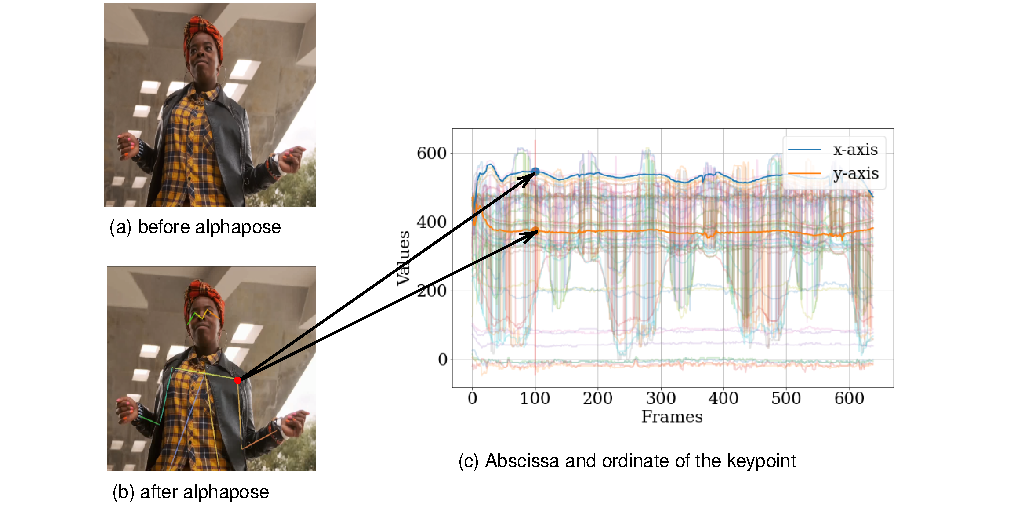
\includegraphics[width=\textwidth]{alphapose_pipeline.pdf}
	\caption{The pipeline of video processing.}
	\label{fig:alphapose_pipeline}
\end{figure}

The experiment is carried on a set of manually collected data. 
It is a collection of key points obtained from a video of a person's movement, as well as accelerometer and gyroscope readings taken from a person's hand.
The pipeline of transforming video into multidimensional time series is shown in figure \ref{fig:alphapose_pipeline}.
In the experiment, a time series forecast is constructed using the detected related components of the time series.

\section{Problem statement}
Let the values of the multivariate time series 
\[ \bS_y(t) = [S_y^1(t), \ldots, S_y^r(t)] \T \]
be available at time points $t = 1, 2, \ldots, n$.
We assume that a set of auxiliary time series $S_x^1(t), \ldots, S_x^m(t)$ affects the values of $\bS_y(t)$.

It is necessary to predict the values of the original time series $\bS_y(t)$ at time points $n+1, \ldots, n+p$.
We assume that the values of the auxiliary time series are available in the time period for which the prediction of the time series $\bS_y(t)$ is carried out.

In order to calculate the future values of a time series, we must determine a functional dependence illustrating the relationship between the past values of $\bS_y(t)$ and the future ones, as well as taking into account the influence of auxiliary time series $S_x^1(t), \ldots, S_x^m(t)$.

\begin{definition}
	\textbf{The} \emph{prediction model} \textbf{with external factors} is a function:
	\begin{equation*}
		\bS_y(t) = \bF(\bS_y(t-1), \ldots, S_x^1(t), \ldots, S_x^m(t), \ldots) + \boldsymbol{\epsilon}_t.
	\end{equation*}
\end{definition}

The algorithm of sequential locally weighted global linear map (SMAP) \cite{sugihara1994nonlinear} is used as a prediction model with external factors.

The quality criterion of the model is its mean-square error:

\begin{equation*}
	\mathcal{Q} = \dfrac{1}{p} \sum\limits_{i=n+1}^{n+p} ||\boldsymbol{\epsilon}_i||^2.
\end{equation*}

The specificity of this problem is that the size $m$ of the time series set is quite large and that among the time series $S_x^1(t), \ldots, S_x^m(t)$ there are many highly correlated ones.
As a result, using the entire set to predict the time series $\bS_y(t)$ leads to poor forecast quality.
Therefore, the following pipeline for predicting the target variable is proposed:

\begin{enumerate}
	\item Train one of the dimensionality reduction methods if it has trainable parameters.
	\item Translate the source data into latent space.
	\item Apply prediction model with external factors to latent data.
	\item (Optional) Decode obtained predictions to the target space.
\end{enumerate}

\begin{figure}[bhtp]
	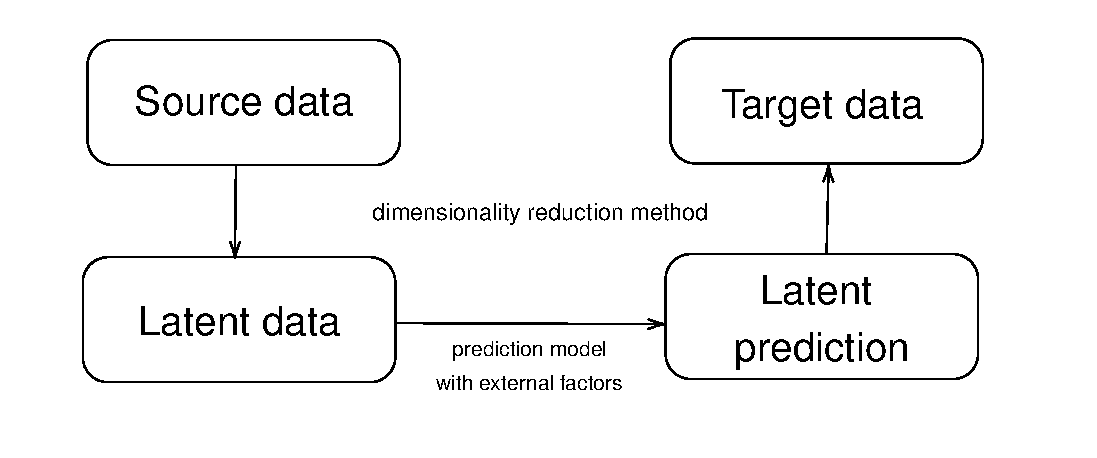
\includegraphics[width=\textwidth]{inference_pipeline}
	\caption{Inference pipeline of the prediction model}
\end{figure}


One way to project source data is to select a fixed number of time series that have the greatest impact on the target variable using the CCM method.
For a pair of time series
\begin{equation*}
	\bigl(S_x^i(t), S_y^j(t) \bigr) \quad i = 1, \ldots, m \quad j = 1, \ldots r
\end{equation*} 
it determines the impact measure of the time series $S_x^i(t)$ on the target variable $S_y^j(t)$.
Next, select the time series from the set with the maximum impact measure.

\subsection{CCM method}
\begin{figure}[bhtp]
	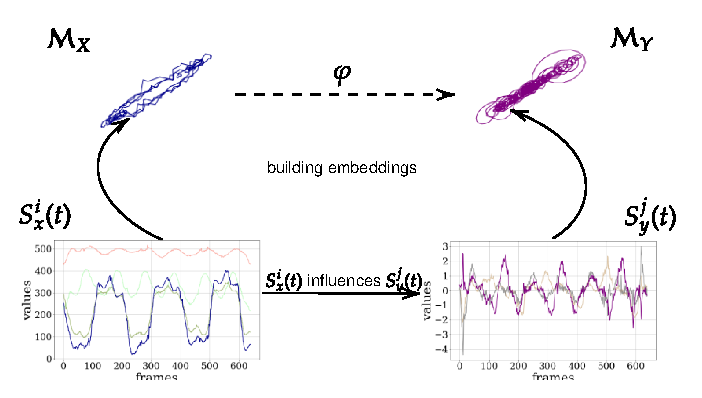
\includegraphics[width=\textwidth]{block_scheme_4.pdf}
	\caption{Application of the CCM method to select the most significant components of a time series}
	\label{fig:schema}
\end{figure}

Let's define the trajectory matrix of the time series $\bx = [x_1, \ldots, x_n]$ as follows:

\begin{equation*} \label{eq:traj_mat}
	\bH_{\bx} = \begin{bmatrix}
		x_1 & x_2 & \ldots & x_{\tau} \\
		x_2 & x_3 & \ldots & x_{\tau+1} \\
		\vdots & \vdots & \ddots & \vdots \\
		x_{N} & x_{N+1} & \ldots & x_n
	\end{bmatrix}, 
\end{equation*} 

where $N$ is the number of delays, $\tau = n - N + 1$.

Denote the $i\text{-th}$ column of the matrix $\bH_{\bx}$ by $\bx_i$.
The matrix $\bH_{\bx}$ takes the form:

\begin{equation*}\label{eq:traj_mat_short}
	\bH_{\bx} = [\bx_1, \ldots, \bx_{\tau}], \qquad \bx_i = [x_i, x_{i+1}, \ldots, x_{i+N-1}] \T
\end{equation*}

Note that all vectors $\bx_t$ belong to the $N-\text{dimensional}$ trajectory space $\dH_{\bx} \subseteq \dR^N$ of the time series $\bx$ and form the phase trajectory $\bx(t) \in \dR^N$.

To detect the relationship between the time series $\bx$ and $\by$, take the element $\bx_0$ from the trajectory space $\dH_{\bx}$ and find $k$ nearest neighbors in the same space. 
Let's denote their time indices (from near to far) by $t_1, \ldots, t_k$.

Since both time series are defined on the same timeline, then we can uniquely obtain the value of the time series $\by$ at time point $t_0 \in \{1, \ldots, n\}$ by the value of the time series $\bx$ and vice versa.
Introduce the mapping from $\dH_{\bx}$ to $\dH_{\by}$ as follows:
$$ \varphi: \bx_0 \mapsto \widehat{\by_0} = \sum\limits_{i=1}^k w_i \by_{t_i}, \qquad 
w_i = \dfrac{u_i}{\sum\limits_{j=1}^k u_j}, \qquad
u_i = \exp \bigl( - \| \bx_0 - \bx_{t_i} \| \bigr).$$

\begin{definition}
	The time series $\bx$ and $\by$ are called \textbf{linked} if the mapping $\varphi$ is Lipschitz:
	$$\rho_{\dH_{\by}}(\varphi(\bx_i), \varphi(\bx_j)) \leq C \rho_{\dH_{\bx}}(\bx_i, \bx_j) \qquad \bx_i, \bx_j \in \dH_{\bx}. $$
\end{definition}

We introduce a metric proximity function of vectors in the vicinity of $U_k(\bx_{t_0})$ and $U_k(\by_{t_0})$ to check for connectivity:

\begin{equation}
	L(\bx, \by) = \dfrac{R(U_k(\bx_{t_0}))}{R(U_k(\by_{t_0}))}, \qquad R(U_k(\bx_{t_0})) = \dfrac{1}{k} \sum\limits_{i=1}^k \rho_{\dH_{\bx}}(\bx_{t_0}, \bx_{t_j}).
\end{equation}

If $L(\bx,\by)$ is greater than the specified threshold, then the time series $\by$ depends on the time series $\bx$.

Another way to project the source data is to use the Pearson correlation coefficient $\text{corr}(\by_0, \widehat{\by_0})$. 
One can choose a fixed amount of mostly correlated auxiliary time series or filter them out using threshold.

\subsection{PLS method}
Another way to solve above stated problem is to reduce the dimension in a consistent manner.
The partial least squares method restores the relationship between the datasets $\bX$ and $\bY$.
The object matrix $\bX$ and the target matrix $\bY$ are projected onto the latent space $\dR^K$ of smaller dimension as follows:
$$ \underset{n \times d}{\bX} = \underset{n \times K}{\bT} \cdot \underset{K \times d}{\bP\T} + \underset{n \times d}{\bE} $$
$$ \underset{n \times s}{\bY} = \underset{n \times K}{\bU} \cdot \underset{K \times s}{\bQ\T} + \underset{n \times s}{\bF}, $$
where $\bT$ and $\bU$ ~--- matrices describing objects and targets in the latent space, $\bP$ and $\bQ$ --- transition matrices from the latent space to the original, $\bE$ and $\bF$ --- remainder matrices.

The source data transformation function has the form:
$$f(\bX) = \bX\bW_{\bx}\qquad g(\bY) = \bY\bW_{\by}, $$
where the weight matrices $\bW_{\bx} \in \dR^{d \times K}$ and $\bW_{\by}\in \dR^{s \times K}$ are found by maximizing the sample covariance:
$$ (\bW_{\bx}, \bW_{\by}) = \underset{\bW_{\bx}, \bW_{\by}}{\text{argmax}}\; \text{Cov}(\bX\bW_{\bx}, \bY\bW_{\by})$$

The PLS algorithm works for previously column-normalized matrices $\bX$ and $\bY$ and the number of components $K$ as follows.
Let's set $\bX_1 = \bX, \: \bY_1 = \bY$.
Next, for each $k \in [1, K]$:
\begin{enumerate}
	\item Calculate $\ba_k\in \dR^d$ and $\bb_k\in \dR^s$, the first left and right singular vectors of the matrix $\bX_k^T\bY_k$; from the definition it follows that $(\ba_k, \bb_k) = \underset{\ba, \bb}{\text{argmax}} \text{Cov} (\bX_k \ba, \bY_k \bb)$.
	\item Project the matrices $\bX_k$ and $\bY_k$ onto singular vectors: $\bt_k = \bX_k \ba_k, \; \bu_k = \bY_k\bb_k$.
	Best rank-one approximation
	\item Regress the matrix $\bX_k$ by the vector $\bt_k$, that is, find the vector $\bp_k$ such that the matrix $\bt_k\bp_k\T$ is the best rank-one approximation of the matrix $\bX_k$ by the Frobenius norm; do the same with the matrix $\bY_k$ and the vector $\bu_k$ and get the vector $\bq_k$.
	\item Subtract from the matrix $\bX_k$ its rank-one approximation from the previous step, denote this matrix $\bX_{k+1}$; similarly, get the matrix $\bY_{k+1}$.
\end{enumerate}

Get an explicit form of the matrices $\bW_{\bx}$ and $\bW_{\by}$ from the PLS algorithm. Note that:
$$\bX\cdot\bA(\bP\T\bA)^{-1} = (\bT\bP\T\bA + \bE\bA)(\bP \T \bA)^{-1} \approx\bT, $$
where the matrices $\bA, \:\bP, \:\bT$ are formed from the columns $\ba_k, \:\bp_k, \:\bt_k$ respectively. 
Similarly, $\bY\cdot\bB(\bQ\T\bB)^{-1} \approx \bU$, where the matrices $\bB, \:\bQ, \:\bU$ are formed from the columns $\bb_k, \:\bq_k, \: \bu_k$, respectively.
Thus:
$$\bW_{\bx} = \bA(\bP\T\bA)^{-1}, \qquad\bW_{\by}= \bB(\bQ\T\bB)^{-1}. $$

\subsection{PLS-Autoencoder and PLS-CCM methods}
The main disadvantage of the classical PLS method is the low quality when working with data that have complex nonlinear dependencies.
For this reason, extensions of the linear PLS method, that transform input data using smooth nonlinear functions, have been developed .

One of such extensions is the PLS-Autoencoder method.
Neural networks act as parametric functions that translate the source data into the latent space and vice versa.
Multilayer perceptrons are used in this work.

\begin{figure}
	\begin{tikzpicture}[scale=1, every node/.style={scale=1}]
		\matrix (m) [matrix of math nodes,row sep=4em,column sep=5em,minimum width=3em]
		{
			\underset{n \times d}{\bX} & \underset{n \times s}{\bY} \\
			\underset{n \times K}{\mathbf{T}} & \underset{n \times K}{\mathbf{U}} \\
		};
		\path[-stealth]
		(m-2-1) edge node [right] {$\varphi_{\text{dec}}$} (m-1-1)
		(m-2-2) edge node [left] {$\psi_{\text{dec}}$} (m-1-2)
		(m-1-1) edge [bend right] node [left] {$\varphi_{\text{enc}}$} (m-2-1)
		(m-1-2) edge [bend left] node [right] {$\psi_{\text{enc}}$} (m-2-2)
		(m-2-1) edge [<->] (m-2-2);
	\end{tikzpicture}
	\qquad
	\begin{tikzpicture}[scale=1, every node/.style={scale=1}]
		\matrix (m) [matrix of math nodes,row sep=4em,column sep=5em,minimum width=3em]
		{
			\underset{n \times d}{\bX} & \underset{n \times s}{\bY} \\
			\underset{n \times K}{\mathbf{T}} & \underset{n \times K}{\mathbf{U}} \\
		};
		\path[-stealth]
		(m-2-1) edge node [right] {$\varphi_{\text{dec}}$} (m-1-1)
		(m-2-2) edge node [left] {$\psi_{\text{dec}}$} (m-1-2)
		(m-1-1) edge [bend right] node [left] {$\varphi_{\text{enc}}$} (m-2-1)
		(m-1-2) edge [bend left] node [right] {$\psi_{\text{enc}}$} (m-2-2)
		(m-2-1) edge [->] node [above] {$CCM_{\mathbf{TU}}$} (m-2-2)
		(m-1-1) edge [->] node [above] {$CCM_{\mathbf{XY}}$} (m-1-2);
	\end{tikzpicture}
	\caption{Left: PLS-Autoencoder, right: PLS-CCM}
\end{figure}

The loss function of this model has the form:
\begin{gather*}
	\mathcal{L} = \lambda_1 \cdot \mathcal{L}^X_{\text{recov}}(\bX, \hat{\bX}) + \lambda_2 \cdot \mathcal{L}^Y_{\text{recov}}(\bY, \hat{\bY}) + \lambda_3 \cdot \mathcal{L}_{\text{cons}}(\bT, \bU), 
	\qquad \lambda_1, \lambda_2, \lambda_3 > 0,	\\
	\mathcal{L}^X_{\text{recov}}(\bX, \hat{\bX}) = \| \bX - \hat{\bX}\|_2^2 \: , \text{ where } \hat{\bX} = \varphi_{\text{dec}}(\varphi_{\text{enc}}(\bX)), \\
	\mathcal{L}^Y_{\text{recov}}(\bY, \hat{\bY}) = \| \bY - \hat{\bY}\|_2^2 \: , \text{ where } \hat{\bY} = \psi_{\text{dec}}(\psi_{\text{enc}}(\bY)), \\
	\mathcal{L}_{\text{cons}}(\bT, \bU) = \dfrac{1}{1 + \left( \frac{1}{n} \, \text{tr}\bigl(\bU_{\text{centered}}\T \bT_{\text{centered}} \bigr) \right)^2}
\end{gather*}
where $\mathcal{L}_{\text{recov}}$ is responsible for how accurately the original data is restored from their projections into the latent space, and $\mathcal{L}_{\text{cons}}$ is responsible for the connectivity of low-dimensional latent representations.

It is worth emphasizing that $\mathcal{L}_{\text{cons}}$ maximizes the sum square of the corresponding features covariance, which are columns of the matrices $\bT$ and $\bU$.
Thus, this method does not take into account the consistency of objects in the latent space, that is, rows of matrices $\bT$ and $\bU$.

The new PLS-CCM method takes into account object consistency using metric functions from the CCM method. It is an extension of PLS-Autoencoder, only a new loss function is added:
$$ \mathcal{L}_\text{oc}(\bX, \bY, \bU, \bT) = \left( CCM_{\mathbf{XY}} - CCM_{\mathbf{TU}} \right)^2 ,$$
where $CCM_{\mathbf{XY}}$ ~--- the value characterizing the quality of approximation $\by_n$ using $\bx_n$ constructed in the trajectory space consisting of the first $n-1$ objects, and $CCM_{\mathbf{TU}}$~--- the same value, obtained from the matrices $\bU$ and $\bT$.

\section{Computational experiment}
The aim of the experiment is to compare different methods of consistent dimensionality reduction of spaces.
These methods are used to predict the trajectory of the hand movement according to the corresponding video sequence.
An important experiment part is the study of the results of the time series prediction model applied to the elements of phase trajectories space and to the elements of the trajectory subspace of a smaller dimension.

\begin{figure}[bhtp]
	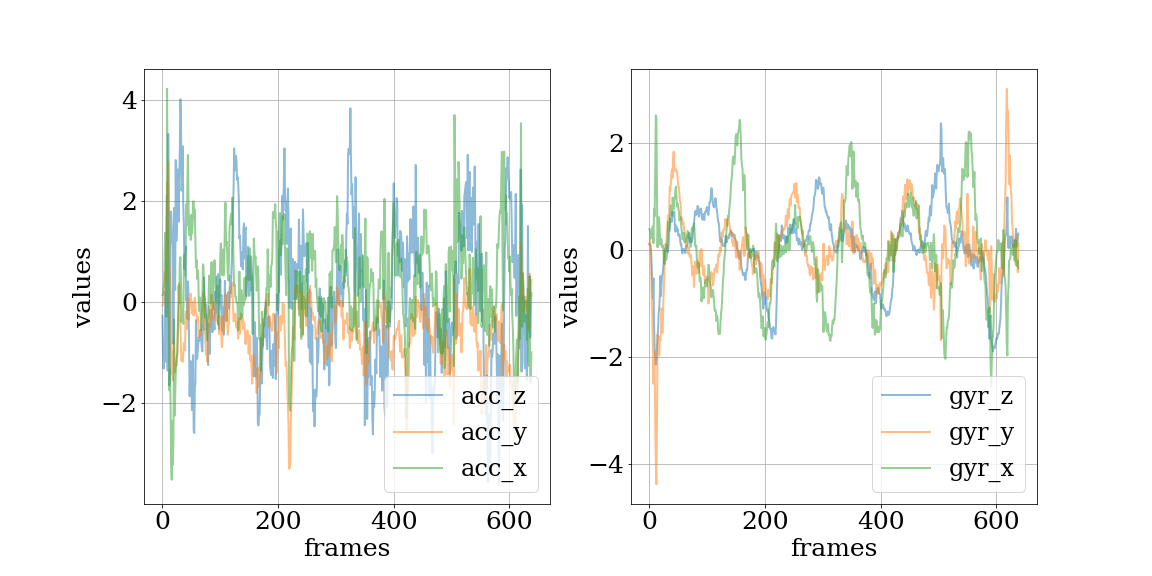
\includegraphics[width=\textwidth]{cyclic_devices_data.png}
	\caption{Accelerometer and gyroscope data obtained by hand movement}
	\label{fig:devices_data}
\end{figure}
The data is a set of videos on which various hand movements (cyclic and chaotic) are performed. 
The data also includes accelerometer and gyroscope readings with a frequency of 100 Hertz, fixed on one of the hands.
These devices form a 6-dimensional time series: The accelerometer and gyroscope show changes in values along the X, Y, and Z axes.
Next, using the alphapose framework \cite{alphapose_fang2017rmpe, alphapose_li2019crowdpose, alphapose_xiu2018poseflow}, the coordinates of the limbs, namely 68 key points, are extracted from the video sequence.
As a result, we obtain a multivariate time series of dimension 136, each component of which shows a change in one of the coordinates of some key point.
Then highly correlated components are excluded from the resulting time series.
After that, the resulting multivariate time series are reduced to one time scale by removing elements of a longer time series.

\begin{figure}[bhtp]
	\centering
	\subfloat[The result of the alphapose framework]{%
		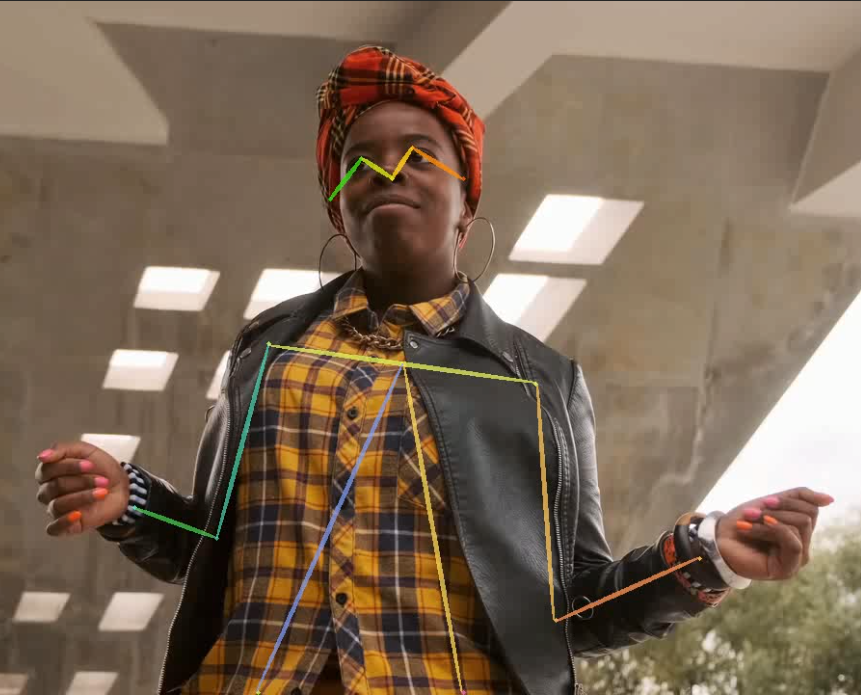
\includegraphics[width=0.45\linewidth]{after_alphapose.png}%
	}
	\subfloat[Keypoints data obtained from the video]{%
		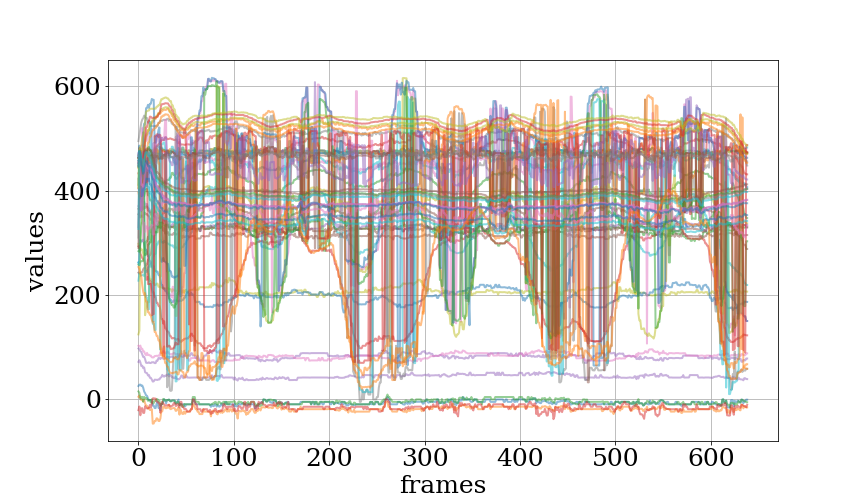
\includegraphics[width=0.45\linewidth]{cyclic_video_data.png}
	}
	\caption{Video processing scheme}
	\label{fig:video_data}
\end{figure}

\section{Error analysis}
\begin{table}[bhtp]
	\fontsize{10pt}{14pt}
	\selectfont
	\centering
	\caption{Comparison of the error (MSE) of the predictive model applied in the trajectory space and in its subspace obtained by CCM}
	\label{tbl:space_and_subspace}
	\begin{tabularx}{\textwidth}{c|XXXXXX}
		\hline
		& acc\_z & acc\_y & acc\_x & gyr\_z & gyr\_y & gyr\_x \\
		\hline
		space & 1.053 $\pm$ 2.223 & 0.401 $\pm$ 0.833 & 0.483 $\pm$ 0.825 & 0.084 $\pm$ 0.537 & 0.090 $\pm$ 0.094 & 0.063 $\pm$ 0.295 \\
		\hline
		subspace & 0.315 $\pm$ 0.461 & 0.043 $\pm$ 0.051 & 0.150 $\pm$ 0.177 & 0.001 $\pm$ 0.001	& 0.015 $\pm$ 0.031 & 0.001 $\pm$ 0.003 \\
		\hline
	\end{tabularx}
\end{table}

To begin with, let's compare the predictions quality of the forecasting model applied in the trajectory space and its subspace.
The table \ref{tbl:space_and_subspace} shows the mean-square error of the predictions of the accelerometer and gyroscope values for each of the axes and their standard deviations.
It shows that the predictive model applied in the trajectory subspace gives more accurate predictions, since most of the features of the original space are uninformative and many of them are highly correlated.

Next, we will consider various methods of dimension reduction of the trajectory space.
5 methods were compared: CCM (K video features are selected that have the greatest impact on one of the accelerometer or gyroscope readings), PLS, CCA, PLS-AE, PLS-CCM.
These methods are applied on two data sets: corresponding to cyclic and arbitrary hand movements.
In the PLS-AE and PLS-CCM methods, a multilayer perceptron with the LeakyReLU activation function is taken as encoding and recovery functions, 

\begin{table}[bhtp]
	\centering
	\caption{The standard deviation between the true readings of the devices and the predictions obtained with one of the dimensionality reduction methods}
	\label{tbl:methods}
	\begin{tabular}{l|c|lllll}
		\hline
		\multicolumn{2}{l}{\diaghead{\hskip4cm}{Target feature}{Method}} \vline & CCM & PLS & CCA & PLS-AE & PLS-CCM \\
		\hline
		\multirow{6}{*}{\rotatebox[origin=c]{90}{cyclic}} & acc\_z & 0.400 & 0.067 & 0.146 & \textbf{0.065} & 0.097 \\
		& acc\_y & \textbf{0.011} & 0.045 & 0.219 & 0.067 & 0.066 \\
		& acc\_x & {0.056} & 0.073 & 0.092 & \textbf{0.045} & 0.054 \\
		& gyr\_z & \textbf{0.001} & 0.034 & 0.105 & 0.031 & 0.018 \\
		& gyr\_y & \textbf{0.002} & 0.023 & 0.010 & 0.024 & 0.070 \\
		& gyr\_x & {0.027} & 0.045 & 0.196 & 0.011 & \textbf{0.009} \\
		\hline
		\multirow{6}{*}{\rotatebox[origin=c]{90}{chaotic}} & acc\_z & 1.015 & \textbf{0.256} & 0.405 & 0.357 & 0.325 \\
		& acc\_y & 0.547 & 0.075 & \textbf{0.036} & 0.155 & 0.156 \\
		& acc\_x & {0.568} & 0.382 & 0.628 & 0.364 & \textbf{0.324} \\
		& gyr\_z & {0.099} & 0.066 & \textbf{0.021} & 0.259 & 0.127 \\
		& gyr\_y & {0.263} & 0.032 & \textbf{0.028} & 0.103 & 0.172 \\
		& gyr\_x & {0.074} & \textbf{0.039} & 0.055 & 0.129 & 0.298 \\
		\hline   
	\end{tabular}
\end{table}

\section{Conclusion}
The paper proposes a method for generalizing the PLS and CCA methods using the Sugihara method by constructing embeddings and choosing a metric for evaluating the quality of approximation.
A computational experiment was carried out on the data of devices and video series.
It was found that the using data from the video improves the forecasting quality.
It is shown that the predictive model is less stable when it is applied in the trajectory space.

In the future, it is planned to apply the method not to two-dimensional data that correspond to regular measurements of a certain value, but to sporadic time series.
This means that the input data will be multi-index matrices.

%%===========================================================================================%%
%% If you are submitting to one of the Nature Portfolio journals, using the eJP submission   %%
%% system, please include the references within the manuscript file itself. You may do this  %%
%% by copying the reference list from your .bbl file, paste it into the main manuscript .tex %%
%% file, and delete the associated \verb+\bibliography+ commands.                            %%
%%=====================================	======================================================%%

\bibliographystyle{bst/sn-mathphys}
\bibliography{sn-bibliography}% common bib file
%% if required, the content of .bbl file can be included here once bbl is generated
%%%%%%%%%%%%%%%%%%%%%%%%%%%%%%%%%%%%%%%%%%%%%%%%%%%%%%%%%%%%%%%%%%%%%%
%%                                                                 %%
%% Please do not use \input{...} to include other tex files.       %%
%% Submit your LaTeX manuscript as one .tex document.              %%
%%                                                                 %%
%% All additional figures and files should be attached             %%
%% separately and not embedded in the \TeX\ document itself.       %%
%%                                                                 %%
%%%%%%%%%%%%%%%%%%%%%%%%%%%%%%%%%%%%%%%%%%%%%%%%%%%%%%%%%%%%%%%%%%%%%

%%\documentclass[referee,sn-basic]{sn-jnl}% referee option is meant for double line spacing

%%=======================================================%%
%% to print line numbers in the margin use lineno option %%
%%=======================================================%%

%%\documentclass[lineno,sn-basic]{sn-jnl}% Basic Springer Nature Reference Style/Chemistry Reference Style

%%======================================================%%
%% to compile with pdflatex/xelatex use pdflatex option %%
%%======================================================%%

%%\documentclass[pdflatex,sn-basic]{sn-jnl}% Basic Springer Nature Reference Style/Chemistry Reference Style

%%\documentclass[sn-basic]{sn-jnl}% Basic Springer Nature Reference Style/Chemistry Reference Style
\documentclass[bst/sn-mathphys]{sn-jnl}% Math and Physical Sciences Reference Style
%%\documentclass[sn-aps]{sn-jnl}% American Physical Society (APS) Reference Style
%%\documentclass[sn-vancouver]{sn-jnl}% Vancouver Reference Style
%%\documentclass[sn-apa]{sn-jnl}% APA Reference Style
%%\documentclass[sn-chicago]{sn-jnl}% Chicago-based Humanities Reference Style
%%\documentclass[sn-standardnature]{sn-jnl}% Standard Nature Portfolio Reference Style
%%\documentclass[default]{sn-jnl}% Default
%%\documentclass[default,iicol]{sn-jnl}% Default with double column layout

%%%% Standard Packages
\usetikzlibrary{matrix}
\usepackage{makecell}
\usepackage{subfig}
\usepackage{tabularx}
\usepackage{tabulary}

\newcommand{\bz}{\mathbf{z}}
\newcommand{\bx}{\ensuremath{\mathbf{x}}}
\newcommand{\by}{\mathbf{y}}
\newcommand{\bv}{\mathbf{v}}
\newcommand{\bw}{\mathbf{w}}
\newcommand{\ba}{\mathbf{a}}
\newcommand{\bb}{\mathbf{b}}
\newcommand{\bp}{\mathbf{p}}
\newcommand{\bq}{\mathbf{q}}
\newcommand{\bt}{\mathbf{t}}
\newcommand{\bu}{\mathbf{u}}
\newcommand{\bT}{\mathbf{T}}
\newcommand{\bX}{\mathbf{X}}
\newcommand{\bZ}{\mathbf{Z}}
\newcommand{\bS}{\mathbf{S}}
\newcommand{\bH}{\mathbf{H}}
\newcommand{\bW}{\mathbf{W}}
\newcommand{\bY}{\mathbf{Y}}
\newcommand{\bU}{\mathbf{U}}
\newcommand{\bQ}{\mathbf{Q}}
\newcommand{\bP}{\mathbf{P}}
\newcommand{\bA}{\mathbf{A}}
\newcommand{\bB}{\mathbf{B}}
\newcommand{\bC}{\mathbf{C}}
\newcommand{\bE}{\mathbf{E}}
\newcommand{\bF}{\mathbf{F}}
\newcommand{\bomega}{\boldsymbol{\omega}}
\newcommand{\btheta}{\boldsymbol{\theta}}
\newcommand{\bgamma}{\boldsymbol{\gamma}}
\newcommand{\bdelta}{\boldsymbol{\delta}}
\newcommand{\bPsi}{\boldsymbol{\Psi}}
\newcommand{\bpsi}{\boldsymbol{\psi}}
\newcommand{\bxi}{\boldsymbol{\xi}}
\newcommand{\bchi}{\boldsymbol{\chi}}
\newcommand{\bzeta}{\boldsymbol{\zeta}}
\newcommand{\blambda}{\boldsymbol{\lambda}}
\newcommand{\beps}{\boldsymbol{\varepsilon}}
\newcommand{\bZeta}{\boldsymbol{Z}}
% mathcal
\newcommand{\cX}{\mathcal{X}}
\newcommand{\cY}{\mathcal{Y}}
\newcommand{\cW}{\mathcal{W}}

\newcommand{\dH}{\mathbb{H}}
\newcommand{\dR}{\mathbb{R}}

\renewcommand{\T}{^{\mathsf{T}}}
%%%%

%%%%%=============================================================================%%%%
%%%%  Remarks: This template is provided to aid authors with the preparation
%%%%  of original research articles intended for submission to journals published 
%%%%  by Springer Nature. The guidance has been prepared in partnership with 
%%%%  production teams to conform to Springer Nature technical requirements. 
%%%%  Editorial and presentation requirements differ among journal portfolios and 
%%%%  research disciplines. You may find sections in this template are irrelevant 
%%%%  to your work and are empowered to omit any such section if allowed by the 
%%%%  journal you intend to submit to. The submission guidelines and policies 
%%%%  of the journal take precedence. A detailed User Manual is available in the 
%%%%  template package for technical guidance.
%%%%%=============================================================================%%%%

\jyear{2022}%

%% as per the requirement new theorem styles can be included as shown below
\theoremstyle{thmstyleone}%
\newtheorem{theorem}{Theorem}%  meant for continuous numbers
%%\newtheorem{theorem}{Theorem}[section]% meant for sectionwise numbers
%% optional argument [theorem] produces theorem numbering sequence instead of independent numbers for Proposition
\newtheorem{proposition}[theorem]{Proposition}% 
%%\newtheorem{proposition}{Proposition}% to get separate numbers for theorem and proposition etc.

\theoremstyle{thmstyletwo}%
\newtheorem{example}{Example}%
\newtheorem{remark}{Remark}%

\theoremstyle{thmstylethree}%
\newtheorem{definition}{Definition}%

\raggedbottom
%%\unnumbered% uncomment this for unnumbered level heads

\begin{document}

\title{Reconstruction of acceleration hand trajectory with video}

%%=============================================================%%
%% Prefix	-> \pfx{Dr}
%% GivenName	-> \fnm{Joergen W.}
%% Particle	-> \spfx{van der} -> surname prefix
%% FamilyName	-> \sur{Ploeg}
%% Suffix	-> \sfx{IV}
%% NatureName	-> \tanm{Poet Laureate} -> Title after name
%% Degrees	-> \dgr{MSc, PhD}
%% \author*[1,2]{\pfx{Dr} \fnm{Joergen W.} \spfx{van der} \sur{Ploeg} \sfx{IV} \tanm{Poet Laureate} 
%%                 \dgr{MSc, PhD}}\email{iauthor@gmail.com}
%%=============================================================%%

\author*[1]{\fnm{Eduard} \sur{Vladimirov}}\email{vladimirov.ea@phystech.edu}

\author[1]{\fnm{Roman} \sur{Isachenko}}\email{roman.isachenko@phystech.edu}
\equalcont{These authors contributed equally to this work.}

\author[1]{\fnm{Vadim} \sur{Strijov}}\email{strijov@phystech.edu}
\equalcont{These authors contributed equally to this work.}

\affil[1]{\orgname{Moscow Institute of Physics and Technology}, \orgaddress{\street{Inststitutskii per.~9}, \city{Dolgoprudny}, \postcode{141700}, \state{Moscow Region}, \country{Russia}}}

%%==================================%%
%% sample for unstructured abstract %%
%%==================================%%

\abstract{This paper investigates the problem of forecasting a time series with a complex structure. 
The complex structure means the presence of non-linear dependencies and a varying period. 
We have to find causal relationships between time series forecasts. 
In order to do this, we reduce the dimension of trajectory spaces.
The paper introduces a new way for the consistent dimensional reduction of time series. 
The proposed method combines the partial least squares method and convergent cross mapping method. 
To demonstrate the results of the work we tackle the problem of hand trajectory reconstruction with video.}

\keywords{Pose estimation, Time series, Phase trajectory, Trajectory subspace, Convergent cross mapping, Partial least squares}
%%\pacs[JEL Classification]{D8, H51}

%%\pacs[MSC Classification]{35A01, 65L10, 65L12, 65L20, 65L70}

\maketitle

\section{Introduction}

In this paper, we solve the problem of forecasting a target time series based on other time series.
The challenge is to detect relationships between time series and exclude unrelated time series from the predictive model.
Solving this problem improves model's quality.

We propose a new method for filtering multivariate time series. 
It's based on the convergent cross mapping method (CCM) or the Sugihara method \cite{Sugihara90, sugihara1990nonlinear},
which outputs the measure of the feature importance.
CCM compares the nearest neighbors in the trajectory space of the time series $\by$ obtained from the time series $\bx$.

To construct a predictive model, one has to use a trajectory matrix (or Hankel matrix) that describes the phase space of a time series.
For example, in the method of singular spectral analysis (SSA) \cite {golyandina2005ssa, golyandina2001analysis, zhigljavsky2010singular, ignatov2016har}, the time series predictive model is based on the spectral decomposition of the trajectory matrix.
In CCM, Hankel matrices are used for checking the presence of a Lipschitz mapping between trajectory spaces.

However, the dimension of the trajectory space may be extremely high, 
which leads to instability of the predictive model.
To reduce the dimension of the trajectory space by mapping a projection of the phase trajectory into some subspace. 
There is no specific way for CCM to select a subspace in which the phase trajectory is approximated.
In the paper \cite{usmanova2020sphere_regr} this problem is solved using spherical regression: the desired subspace is defined by the set of empirical directions $\{ \bx_i - \bx_j \mid i < j \}$, where $\bx_i \text{~--- elements of the trajectory space}$. 
In the work \cite{alexandrov2005automatic} automatic selection of a pair of principal components is used.
The main idea is to compare the spectral densities of the principal components. 
A simple iteration over the principal components \cite{usmanova2019dependencies} is also used.

The partial least squares method (PLS) \cite{rosipal2005overview, sun2019application} is a popular algorithm for dimensionality reduction problem. It selects the most significant features and builds new ones as their linear combination.
This allows us to obtain a simple, accurate and stable predictive model.
The canonical correlation analysis (CCA) \cite{hardoon2004canonical} is another dimensionality reduction method, which is used in medicine \cite{sadoughi2016application}, gait recognition \cite{xing2016complete} and speech enhancement \cite{benesty2018canonical}. 
It is similar to PLS except that the PLS method maximizes the covariance between projections, and the CCA method — correlation.
The disadvantage of these models is the low accuracy in estimating nonlinear dependencies between data.
The nonlinear extensions of PLS \cite{qin1992nonlinear, rosipal2011nonlinear} have been proposed.
This article uses the PLS-Autoencoder model \cite{wiering2013neural}, which converts the source data using autoencoders.

\begingroup
\renewcommand{\arraystretch}{1.5}
\begin{table}[bhtp]
	\caption{Comparison of the dimensionality reduction methods}
	\label{tbl:dim_reduction_review}
	\begin{tabulary}{\textwidth}{L|L|L|L}
		\hline
		Method name & Advantages & Disadvantages & Loss function \\
		\hline
		Projection to Latent Space methods (PLS, CCA) & Resistance to
		highly correlated features and noise in the data & Poor prediction quality when working with data with non-linear dependencies & No \\
		\hline
		Multiview (iteration through subspaces) & Simplicity of idea and implementation & Huge amount of time & No\\
%		\hline
%		Selection of a pair of principal components & TODO & TODO & No \\
		\hline
		Nonlinear extensions of PLS (PLS-Autoencoder, PLS-CCM) & Higher generalizing ability & More hyperparameters, less resistant to data noise & Yes \\
		\hline
	\end{tabulary}
\end{table}
\endgroup

This paper shows how to apply CCM to reduce the dimension of the trajectory space and how to combine the ideas of the PLS and CCM methods.
To achieve the latter goal, a new loss function for the consistency of latent projections has been introduced.

\begin{figure}
	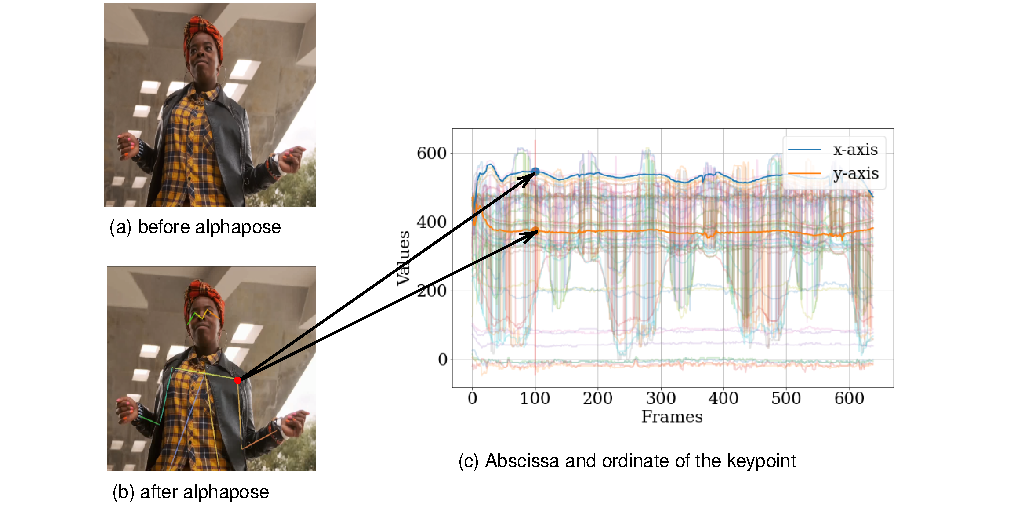
\includegraphics[width=\textwidth]{alphapose_pipeline.pdf}
	\caption{The pipeline of video processing.}
	\label{fig:alphapose_pipeline}
\end{figure}

The experiment is carried on a set of manually collected data. 
It is a collection of key points obtained from a video of a person's movement, as well as accelerometer and gyroscope readings taken from a person's hand.
The pipeline of transforming video into multidimensional time series is shown in figure \ref{fig:alphapose_pipeline}.
In the experiment, a time series forecast is constructed using the detected related components of the time series.

\section{Problem statement}
Let the values of the multivariate time series 
\[ \bS_y(t) = [S_y^1(t), \ldots, S_y^r(t)] \T \]
be available at time points $t = 1, 2, \ldots, n$.
We assume that a set of auxiliary time series $S_x^1(t), \ldots, S_x^m(t)$ affects the values of $\bS_y(t)$.

It is necessary to predict the values of the original time series $\bS_y(t)$ at time points $n+1, \ldots, n+p$.
We assume that the values of the auxiliary time series are available in the time period for which the prediction of the time series $\bS_y(t)$ is carried out.

In order to calculate the future values of a time series, we must determine a functional dependence illustrating the relationship between the past values of $\bS_y(t)$ and the future ones, as well as taking into account the influence of auxiliary time series $S_x^1(t), \ldots, S_x^m(t)$.

\begin{definition}
	\textbf{The} \emph{prediction model} \textbf{with external factors} is a function:
	\begin{equation*}
		\bS_y(t) = \bF(\bS_y(t-1), \ldots, S_x^1(t), \ldots, S_x^m(t), \ldots) + \boldsymbol{\epsilon}_t.
	\end{equation*}
\end{definition}

The algorithm of sequential locally weighted global linear map (SMAP) \cite{sugihara1994nonlinear} is used as a prediction model with external factors.

The quality criterion of the model is its mean-square error:

\begin{equation*}
	\mathcal{Q} = \dfrac{1}{p} \sum\limits_{i=n+1}^{n+p} ||\boldsymbol{\epsilon}_i||^2.
\end{equation*}

The specificity of this problem is that the size $m$ of the time series set is quite large and that among the time series $S_x^1(t), \ldots, S_x^m(t)$ there are many highly correlated ones.
As a result, using the entire set to predict the time series $\bS_y(t)$ leads to poor forecast quality.
Therefore, the following pipeline for predicting the target variable is proposed:

\begin{enumerate}
	\item Train one of the dimensionality reduction methods if it has trainable parameters.
	\item Translate the source data into latent space.
	\item Apply prediction model with external factors to latent data.
	\item (Optional) Decode obtained predictions to the target space.
\end{enumerate}

\begin{figure}[bhtp]
	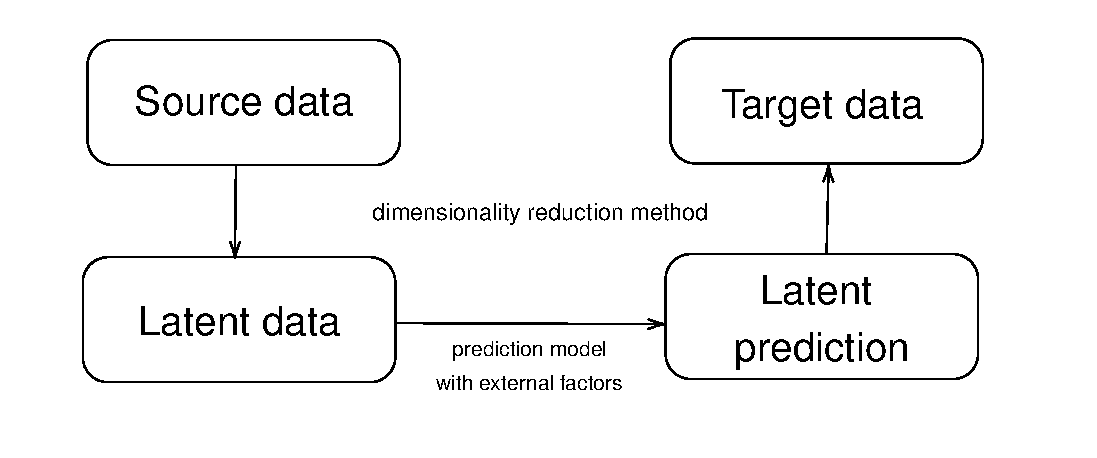
\includegraphics[width=\textwidth]{inference_pipeline}
	\caption{Inference pipeline of the prediction model}
\end{figure}


One way to project source data is to select a fixed number of time series that have the greatest impact on the target variable using the CCM method.
For a pair of time series
\begin{equation*}
	\bigl(S_x^i(t), S_y^j(t) \bigr) \quad i = 1, \ldots, m \quad j = 1, \ldots r
\end{equation*} 
it determines the impact measure of the time series $S_x^i(t)$ on the target variable $S_y^j(t)$.
Next, select the time series from the set with the maximum impact measure.

\subsection{CCM method}
\begin{figure}[bhtp]
	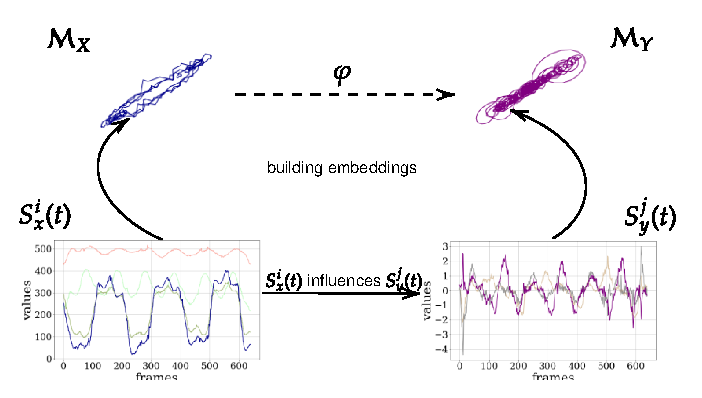
\includegraphics[width=\textwidth]{block_scheme_4.pdf}
	\caption{Application of the CCM method to select the most significant components of a time series}
	\label{fig:schema}
\end{figure}

Let's define the trajectory matrix of the time series $\bx = [x_1, \ldots, x_n]$ as follows:

\begin{equation*} \label{eq:traj_mat}
	\bH_{\bx} = \begin{bmatrix}
		x_1 & x_2 & \ldots & x_{\tau} \\
		x_2 & x_3 & \ldots & x_{\tau+1} \\
		\vdots & \vdots & \ddots & \vdots \\
		x_{N} & x_{N+1} & \ldots & x_n
	\end{bmatrix}, 
\end{equation*} 

where $N$ is the number of delays, $\tau = n - N + 1$.

Denote the $i\text{-th}$ column of the matrix $\bH_{\bx}$ by $\bx_i$.
The matrix $\bH_{\bx}$ takes the form:

\begin{equation*}\label{eq:traj_mat_short}
	\bH_{\bx} = [\bx_1, \ldots, \bx_{\tau}], \qquad \bx_i = [x_i, x_{i+1}, \ldots, x_{i+N-1}] \T
\end{equation*}

Note that all vectors $\bx_t$ belong to the $N-\text{dimensional}$ trajectory space $\dH_{\bx} \subseteq \dR^N$ of the time series $\bx$ and form the phase trajectory $\bx(t) \in \dR^N$.

To detect the relationship between the time series $\bx$ and $\by$, take the element $\bx_0$ from the trajectory space $\dH_{\bx}$ and find $k$ nearest neighbors in the same space. 
Let's denote their time indices (from near to far) by $t_1, \ldots, t_k$.

Since both time series are defined on the same timeline, then we can uniquely obtain the value of the time series $\by$ at time point $t_0 \in \{1, \ldots, n\}$ by the value of the time series $\bx$ and vice versa.
Introduce the mapping from $\dH_{\bx}$ to $\dH_{\by}$ as follows:
$$ \varphi: \bx_0 \mapsto \widehat{\by_0} = \sum\limits_{i=1}^k w_i \by_{t_i}, \qquad 
w_i = \dfrac{u_i}{\sum\limits_{j=1}^k u_j}, \qquad
u_i = \exp \bigl( - \| \bx_0 - \bx_{t_i} \| \bigr).$$

\begin{definition}
	The time series $\bx$ and $\by$ are called \textbf{linked} if the mapping $\varphi$ is Lipschitz:
	$$\rho_{\dH_{\by}}(\varphi(\bx_i), \varphi(\bx_j)) \leq C \rho_{\dH_{\bx}}(\bx_i, \bx_j) \qquad \bx_i, \bx_j \in \dH_{\bx}. $$
\end{definition}

We introduce a metric proximity function of vectors in the vicinity of $U_k(\bx_{t_0})$ and $U_k(\by_{t_0})$ to check for connectivity:

\begin{equation}
	L(\bx, \by) = \dfrac{R(U_k(\bx_{t_0}))}{R(U_k(\by_{t_0}))}, \qquad R(U_k(\bx_{t_0})) = \dfrac{1}{k} \sum\limits_{i=1}^k \rho_{\dH_{\bx}}(\bx_{t_0}, \bx_{t_j}).
\end{equation}

If $L(\bx,\by)$ is greater than the specified threshold, then the time series $\by$ depends on the time series $\bx$.

Another way to project the source data is to use the Pearson correlation coefficient $\text{corr}(\by_0, \widehat{\by_0})$. 
One can choose a fixed amount of mostly correlated auxiliary time series or filter them out using threshold.

\subsection{PLS method}
Another way to solve above stated problem is to reduce the dimension in a consistent manner.
The partial least squares method restores the relationship between the datasets $\bX$ and $\bY$.
The object matrix $\bX$ and the target matrix $\bY$ are projected onto the latent space $\dR^K$ of smaller dimension as follows:
$$ \underset{n \times d}{\bX} = \underset{n \times K}{\bT} \cdot \underset{K \times d}{\bP\T} + \underset{n \times d}{\bE} $$
$$ \underset{n \times s}{\bY} = \underset{n \times K}{\bU} \cdot \underset{K \times s}{\bQ\T} + \underset{n \times s}{\bF}, $$
where $\bT$ and $\bU$ ~--- matrices describing objects and targets in the latent space, $\bP$ and $\bQ$ --- transition matrices from the latent space to the original, $\bE$ and $\bF$ --- remainder matrices.

The source data transformation function has the form:
$$f(\bX) = \bX\bW_{\bx}\qquad g(\bY) = \bY\bW_{\by}, $$
where the weight matrices $\bW_{\bx} \in \dR^{d \times K}$ and $\bW_{\by}\in \dR^{s \times K}$ are found by maximizing the sample covariance:
$$ (\bW_{\bx}, \bW_{\by}) = \underset{\bW_{\bx}, \bW_{\by}}{\text{argmax}}\; \text{Cov}(\bX\bW_{\bx}, \bY\bW_{\by})$$

The PLS algorithm works for previously column-normalized matrices $\bX$ and $\bY$ and the number of components $K$ as follows.
Let's set $\bX_1 = \bX, \: \bY_1 = \bY$.
Next, for each $k \in [1, K]$:
\begin{enumerate}
	\item Calculate $\ba_k\in \dR^d$ and $\bb_k\in \dR^s$, the first left and right singular vectors of the matrix $\bX_k^T\bY_k$; from the definition it follows that $(\ba_k, \bb_k) = \underset{\ba, \bb}{\text{argmax}} \text{Cov} (\bX_k \ba, \bY_k \bb)$.
	\item Project the matrices $\bX_k$ and $\bY_k$ onto singular vectors: $\bt_k = \bX_k \ba_k, \; \bu_k = \bY_k\bb_k$.
	Best rank-one approximation
	\item Regress the matrix $\bX_k$ by the vector $\bt_k$, that is, find the vector $\bp_k$ such that the matrix $\bt_k\bp_k\T$ is the best rank-one approximation of the matrix $\bX_k$ by the Frobenius norm; do the same with the matrix $\bY_k$ and the vector $\bu_k$ and get the vector $\bq_k$.
	\item Subtract from the matrix $\bX_k$ its rank-one approximation from the previous step, denote this matrix $\bX_{k+1}$; similarly, get the matrix $\bY_{k+1}$.
\end{enumerate}

Get an explicit form of the matrices $\bW_{\bx}$ and $\bW_{\by}$ from the PLS algorithm. Note that:
$$\bX\cdot\bA(\bP\T\bA)^{-1} = (\bT\bP\T\bA + \bE\bA)(\bP \T \bA)^{-1} \approx\bT, $$
where the matrices $\bA, \:\bP, \:\bT$ are formed from the columns $\ba_k, \:\bp_k, \:\bt_k$ respectively. 
Similarly, $\bY\cdot\bB(\bQ\T\bB)^{-1} \approx \bU$, where the matrices $\bB, \:\bQ, \:\bU$ are formed from the columns $\bb_k, \:\bq_k, \: \bu_k$, respectively.
Thus:
$$\bW_{\bx} = \bA(\bP\T\bA)^{-1}, \qquad\bW_{\by}= \bB(\bQ\T\bB)^{-1}. $$

\subsection{PLS-Autoencoder and PLS-CCM methods}
The main disadvantage of the classical PLS method is the low quality when working with data that have complex nonlinear dependencies.
For this reason, extensions of the linear PLS method, that transform input data using smooth nonlinear functions, have been developed .

One of such extensions is the PLS-Autoencoder method.
Neural networks act as parametric functions that translate the source data into the latent space and vice versa.
Multilayer perceptrons are used in this work.

\begin{figure}
	\begin{tikzpicture}[scale=1, every node/.style={scale=1}]
		\matrix (m) [matrix of math nodes,row sep=4em,column sep=5em,minimum width=3em]
		{
			\underset{n \times d}{\bX} & \underset{n \times s}{\bY} \\
			\underset{n \times K}{\mathbf{T}} & \underset{n \times K}{\mathbf{U}} \\
		};
		\path[-stealth]
		(m-2-1) edge node [right] {$\varphi_{\text{dec}}$} (m-1-1)
		(m-2-2) edge node [left] {$\psi_{\text{dec}}$} (m-1-2)
		(m-1-1) edge [bend right] node [left] {$\varphi_{\text{enc}}$} (m-2-1)
		(m-1-2) edge [bend left] node [right] {$\psi_{\text{enc}}$} (m-2-2)
		(m-2-1) edge [<->] (m-2-2);
	\end{tikzpicture}
	\qquad
	\begin{tikzpicture}[scale=1, every node/.style={scale=1}]
		\matrix (m) [matrix of math nodes,row sep=4em,column sep=5em,minimum width=3em]
		{
			\underset{n \times d}{\bX} & \underset{n \times s}{\bY} \\
			\underset{n \times K}{\mathbf{T}} & \underset{n \times K}{\mathbf{U}} \\
		};
		\path[-stealth]
		(m-2-1) edge node [right] {$\varphi_{\text{dec}}$} (m-1-1)
		(m-2-2) edge node [left] {$\psi_{\text{dec}}$} (m-1-2)
		(m-1-1) edge [bend right] node [left] {$\varphi_{\text{enc}}$} (m-2-1)
		(m-1-2) edge [bend left] node [right] {$\psi_{\text{enc}}$} (m-2-2)
		(m-2-1) edge [->] node [above] {$CCM_{\mathbf{TU}}$} (m-2-2)
		(m-1-1) edge [->] node [above] {$CCM_{\mathbf{XY}}$} (m-1-2);
	\end{tikzpicture}
	\caption{Left: PLS-Autoencoder, right: PLS-CCM}
\end{figure}

The loss function of this model has the form:
\begin{gather*}
	\mathcal{L} = \lambda_1 \cdot \mathcal{L}^X_{\text{recov}}(\bX, \hat{\bX}) + \lambda_2 \cdot \mathcal{L}^Y_{\text{recov}}(\bY, \hat{\bY}) + \lambda_3 \cdot \mathcal{L}_{\text{cons}}(\bT, \bU), 
	\qquad \lambda_1, \lambda_2, \lambda_3 > 0,	\\
	\mathcal{L}^X_{\text{recov}}(\bX, \hat{\bX}) = \| \bX - \hat{\bX}\|_2^2 \: , \text{ where } \hat{\bX} = \varphi_{\text{dec}}(\varphi_{\text{enc}}(\bX)), \\
	\mathcal{L}^Y_{\text{recov}}(\bY, \hat{\bY}) = \| \bY - \hat{\bY}\|_2^2 \: , \text{ where } \hat{\bY} = \psi_{\text{dec}}(\psi_{\text{enc}}(\bY)), \\
	\mathcal{L}_{\text{cons}}(\bT, \bU) = \dfrac{1}{1 + \left( \frac{1}{n} \, \text{tr}\bigl(\bU_{\text{centered}}\T \bT_{\text{centered}} \bigr) \right)^2}
\end{gather*}
where $\mathcal{L}_{\text{recov}}$ is responsible for how accurately the original data is restored from their projections into the latent space, and $\mathcal{L}_{\text{cons}}$ is responsible for the connectivity of low-dimensional latent representations.

It is worth emphasizing that $\mathcal{L}_{\text{cons}}$ maximizes the sum square of the corresponding features covariance, which are columns of the matrices $\bT$ and $\bU$.
Thus, this method does not take into account the consistency of objects in the latent space, that is, rows of matrices $\bT$ and $\bU$.

The new PLS-CCM method takes into account object consistency using metric functions from the CCM method. It is an extension of PLS-Autoencoder, only a new loss function is added:
$$ \mathcal{L}_\text{oc}(\bX, \bY, \bU, \bT) = \left( CCM_{\mathbf{XY}} - CCM_{\mathbf{TU}} \right)^2 ,$$
where $CCM_{\mathbf{XY}}$ ~--- the value characterizing the quality of approximation $\by_n$ using $\bx_n$ constructed in the trajectory space consisting of the first $n-1$ objects, and $CCM_{\mathbf{TU}}$~--- the same value, obtained from the matrices $\bU$ and $\bT$.

\section{Computational experiment}
The aim of the experiment is to compare different methods of consistent dimensionality reduction of spaces.
These methods are used to predict the trajectory of the hand movement according to the corresponding video sequence.
An important experiment part is the study of the results of the time series prediction model applied to the elements of phase trajectories space and to the elements of the trajectory subspace of a smaller dimension.

\begin{figure}[bhtp]
	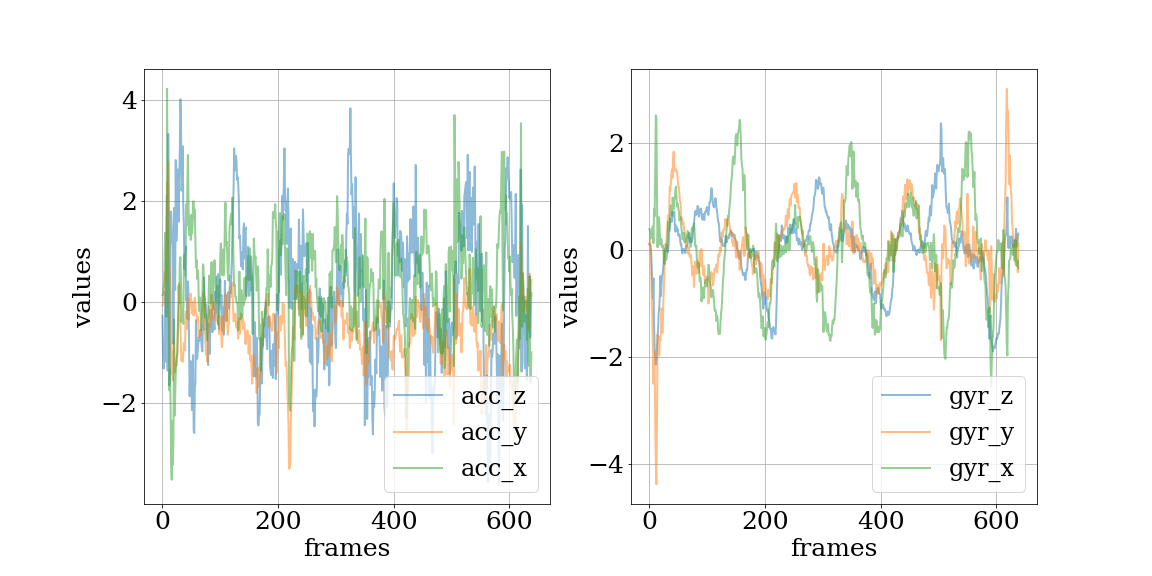
\includegraphics[width=\textwidth]{cyclic_devices_data.png}
	\caption{Accelerometer and gyroscope data obtained by hand movement}
	\label{fig:devices_data}
\end{figure}
The data is a set of videos on which various hand movements (cyclic and chaotic) are performed. 
The data also includes accelerometer and gyroscope readings with a frequency of 100 Hertz, fixed on one of the hands.
These devices form a 6-dimensional time series: The accelerometer and gyroscope show changes in values along the X, Y, and Z axes.
Next, using the alphapose framework \cite{alphapose_fang2017rmpe, alphapose_li2019crowdpose, alphapose_xiu2018poseflow}, the coordinates of the limbs, namely 68 key points, are extracted from the video sequence.
As a result, we obtain a multivariate time series of dimension 136, each component of which shows a change in one of the coordinates of some key point.
Then highly correlated components are excluded from the resulting time series.
After that, the resulting multivariate time series are reduced to one time scale by removing elements of a longer time series.

\begin{figure}[bhtp]
	\centering
	\subfloat[The result of the alphapose framework]{%
		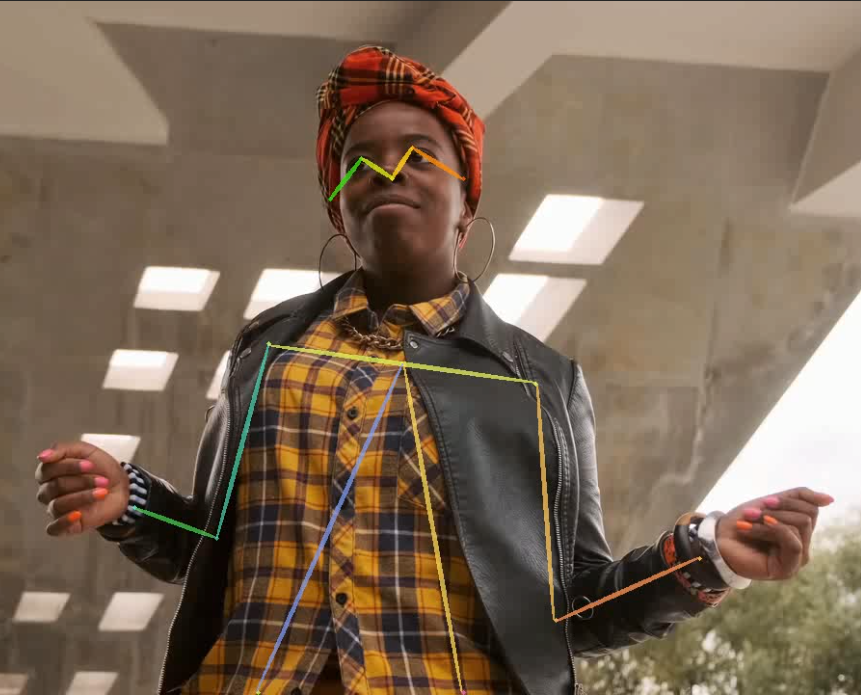
\includegraphics[width=0.45\linewidth]{after_alphapose.png}%
	}
	\subfloat[Keypoints data obtained from the video]{%
		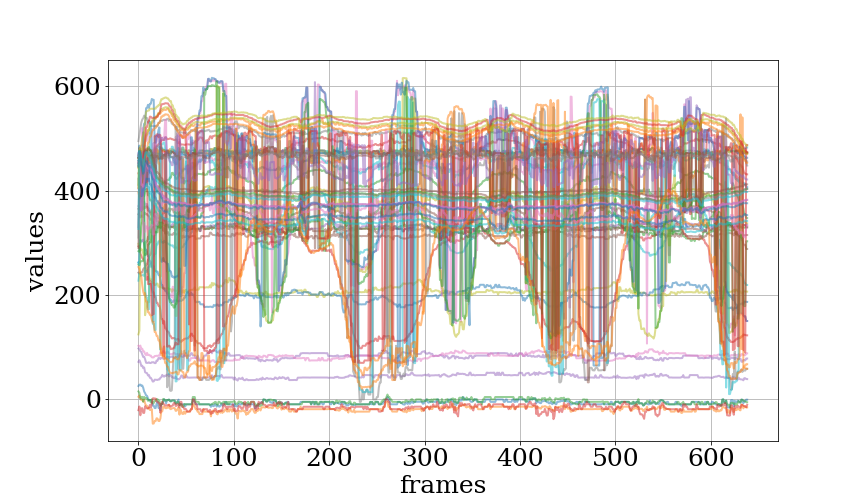
\includegraphics[width=0.45\linewidth]{cyclic_video_data.png}
	}
	\caption{Video processing scheme}
	\label{fig:video_data}
\end{figure}

\section{Error analysis}
\begin{table}[bhtp]
	\fontsize{10pt}{14pt}
	\selectfont
	\centering
	\caption{Comparison of the error (MSE) of the predictive model applied in the trajectory space and in its subspace obtained by CCM}
	\label{tbl:space_and_subspace}
	\begin{tabularx}{\textwidth}{c|XXXXXX}
		\hline
		& acc\_z & acc\_y & acc\_x & gyr\_z & gyr\_y & gyr\_x \\
		\hline
		space & 1.053 $\pm$ 2.223 & 0.401 $\pm$ 0.833 & 0.483 $\pm$ 0.825 & 0.084 $\pm$ 0.537 & 0.090 $\pm$ 0.094 & 0.063 $\pm$ 0.295 \\
		\hline
		subspace & 0.315 $\pm$ 0.461 & 0.043 $\pm$ 0.051 & 0.150 $\pm$ 0.177 & 0.001 $\pm$ 0.001	& 0.015 $\pm$ 0.031 & 0.001 $\pm$ 0.003 \\
		\hline
	\end{tabularx}
\end{table}

To begin with, let's compare the predictions quality of the forecasting model applied in the trajectory space and its subspace.
The table \ref{tbl:space_and_subspace} shows the mean-square error of the predictions of the accelerometer and gyroscope values for each of the axes and their standard deviations.
It shows that the predictive model applied in the trajectory subspace gives more accurate predictions, since most of the features of the original space are uninformative and many of them are highly correlated.

Next, we will consider various methods of dimension reduction of the trajectory space.
5 methods were compared: CCM (K video features are selected that have the greatest impact on one of the accelerometer or gyroscope readings), PLS, CCA, PLS-AE, PLS-CCM.
These methods are applied on two data sets: corresponding to cyclic and arbitrary hand movements.
In the PLS-AE and PLS-CCM methods, a multilayer perceptron with the LeakyReLU activation function is taken as encoding and recovery functions, 

\begin{table}[bhtp]
	\centering
	\caption{The standard deviation between the true readings of the devices and the predictions obtained with one of the dimensionality reduction methods}
	\label{tbl:methods}
	\begin{tabular}{l|c|lllll}
		\hline
		\multicolumn{2}{l}{\diaghead{\hskip4cm}{Target feature}{Method}} \vline & CCM & PLS & CCA & PLS-AE & PLS-CCM \\
		\hline
		\multirow{6}{*}{\rotatebox[origin=c]{90}{cyclic}} & acc\_z & 0.400 & 0.067 & 0.146 & \textbf{0.065} & 0.097 \\
		& acc\_y & \textbf{0.011} & 0.045 & 0.219 & 0.067 & 0.066 \\
		& acc\_x & {0.056} & 0.073 & 0.092 & \textbf{0.045} & 0.054 \\
		& gyr\_z & \textbf{0.001} & 0.034 & 0.105 & 0.031 & 0.018 \\
		& gyr\_y & \textbf{0.002} & 0.023 & 0.010 & 0.024 & 0.070 \\
		& gyr\_x & {0.027} & 0.045 & 0.196 & 0.011 & \textbf{0.009} \\
		\hline
		\multirow{6}{*}{\rotatebox[origin=c]{90}{chaotic}} & acc\_z & 1.015 & \textbf{0.256} & 0.405 & 0.357 & 0.325 \\
		& acc\_y & 0.547 & 0.075 & \textbf{0.036} & 0.155 & 0.156 \\
		& acc\_x & {0.568} & 0.382 & 0.628 & 0.364 & \textbf{0.324} \\
		& gyr\_z & {0.099} & 0.066 & \textbf{0.021} & 0.259 & 0.127 \\
		& gyr\_y & {0.263} & 0.032 & \textbf{0.028} & 0.103 & 0.172 \\
		& gyr\_x & {0.074} & \textbf{0.039} & 0.055 & 0.129 & 0.298 \\
		\hline   
	\end{tabular}
\end{table}

\section{Conclusion}
The paper proposes a method for generalizing the PLS and CCA methods using the Sugihara method by constructing embeddings and choosing a metric for evaluating the quality of approximation.
A computational experiment was carried out on the data of devices and video series.
It was found that the using data from the video improves the forecasting quality.
It is shown that the predictive model is less stable when it is applied in the trajectory space.

In the future, it is planned to apply the method not to two-dimensional data that correspond to regular measurements of a certain value, but to sporadic time series.
This means that the input data will be multi-index matrices.

%%===========================================================================================%%
%% If you are submitting to one of the Nature Portfolio journals, using the eJP submission   %%
%% system, please include the references within the manuscript file itself. You may do this  %%
%% by copying the reference list from your .bbl file, paste it into the main manuscript .tex %%
%% file, and delete the associated \verb+\bibliography+ commands.                            %%
%%=====================================	======================================================%%

\bibliographystyle{bst/sn-mathphys}
\bibliography{sn-bibliography}% common bib file
%% if required, the content of .bbl file can be included here once bbl is generated
%%%%%%%%%%%%%%%%%%%%%%%%%%%%%%%%%%%%%%%%%%%%%%%%%%%%%%%%%%%%%%%%%%%%%%
%%                                                                 %%
%% Please do not use \input{...} to include other tex files.       %%
%% Submit your LaTeX manuscript as one .tex document.              %%
%%                                                                 %%
%% All additional figures and files should be attached             %%
%% separately and not embedded in the \TeX\ document itself.       %%
%%                                                                 %%
%%%%%%%%%%%%%%%%%%%%%%%%%%%%%%%%%%%%%%%%%%%%%%%%%%%%%%%%%%%%%%%%%%%%%

%%\documentclass[referee,sn-basic]{sn-jnl}% referee option is meant for double line spacing

%%=======================================================%%
%% to print line numbers in the margin use lineno option %%
%%=======================================================%%

%%\documentclass[lineno,sn-basic]{sn-jnl}% Basic Springer Nature Reference Style/Chemistry Reference Style

%%======================================================%%
%% to compile with pdflatex/xelatex use pdflatex option %%
%%======================================================%%

%%\documentclass[pdflatex,sn-basic]{sn-jnl}% Basic Springer Nature Reference Style/Chemistry Reference Style

%%\documentclass[sn-basic]{sn-jnl}% Basic Springer Nature Reference Style/Chemistry Reference Style
\documentclass[bst/sn-mathphys]{sn-jnl}% Math and Physical Sciences Reference Style
%%\documentclass[sn-aps]{sn-jnl}% American Physical Society (APS) Reference Style
%%\documentclass[sn-vancouver]{sn-jnl}% Vancouver Reference Style
%%\documentclass[sn-apa]{sn-jnl}% APA Reference Style
%%\documentclass[sn-chicago]{sn-jnl}% Chicago-based Humanities Reference Style
%%\documentclass[sn-standardnature]{sn-jnl}% Standard Nature Portfolio Reference Style
%%\documentclass[default]{sn-jnl}% Default
%%\documentclass[default,iicol]{sn-jnl}% Default with double column layout

%%%% Standard Packages
\usetikzlibrary{matrix}
\usepackage{makecell}
\usepackage{subfig}
\usepackage{tabularx}
\usepackage{tabulary}

\newcommand{\bz}{\mathbf{z}}
\newcommand{\bx}{\ensuremath{\mathbf{x}}}
\newcommand{\by}{\mathbf{y}}
\newcommand{\bv}{\mathbf{v}}
\newcommand{\bw}{\mathbf{w}}
\newcommand{\ba}{\mathbf{a}}
\newcommand{\bb}{\mathbf{b}}
\newcommand{\bp}{\mathbf{p}}
\newcommand{\bq}{\mathbf{q}}
\newcommand{\bt}{\mathbf{t}}
\newcommand{\bu}{\mathbf{u}}
\newcommand{\bT}{\mathbf{T}}
\newcommand{\bX}{\mathbf{X}}
\newcommand{\bZ}{\mathbf{Z}}
\newcommand{\bS}{\mathbf{S}}
\newcommand{\bH}{\mathbf{H}}
\newcommand{\bW}{\mathbf{W}}
\newcommand{\bY}{\mathbf{Y}}
\newcommand{\bU}{\mathbf{U}}
\newcommand{\bQ}{\mathbf{Q}}
\newcommand{\bP}{\mathbf{P}}
\newcommand{\bA}{\mathbf{A}}
\newcommand{\bB}{\mathbf{B}}
\newcommand{\bC}{\mathbf{C}}
\newcommand{\bE}{\mathbf{E}}
\newcommand{\bF}{\mathbf{F}}
\newcommand{\bomega}{\boldsymbol{\omega}}
\newcommand{\btheta}{\boldsymbol{\theta}}
\newcommand{\bgamma}{\boldsymbol{\gamma}}
\newcommand{\bdelta}{\boldsymbol{\delta}}
\newcommand{\bPsi}{\boldsymbol{\Psi}}
\newcommand{\bpsi}{\boldsymbol{\psi}}
\newcommand{\bxi}{\boldsymbol{\xi}}
\newcommand{\bchi}{\boldsymbol{\chi}}
\newcommand{\bzeta}{\boldsymbol{\zeta}}
\newcommand{\blambda}{\boldsymbol{\lambda}}
\newcommand{\beps}{\boldsymbol{\varepsilon}}
\newcommand{\bZeta}{\boldsymbol{Z}}
% mathcal
\newcommand{\cX}{\mathcal{X}}
\newcommand{\cY}{\mathcal{Y}}
\newcommand{\cW}{\mathcal{W}}

\newcommand{\dH}{\mathbb{H}}
\newcommand{\dR}{\mathbb{R}}

\renewcommand{\T}{^{\mathsf{T}}}
%%%%

%%%%%=============================================================================%%%%
%%%%  Remarks: This template is provided to aid authors with the preparation
%%%%  of original research articles intended for submission to journals published 
%%%%  by Springer Nature. The guidance has been prepared in partnership with 
%%%%  production teams to conform to Springer Nature technical requirements. 
%%%%  Editorial and presentation requirements differ among journal portfolios and 
%%%%  research disciplines. You may find sections in this template are irrelevant 
%%%%  to your work and are empowered to omit any such section if allowed by the 
%%%%  journal you intend to submit to. The submission guidelines and policies 
%%%%  of the journal take precedence. A detailed User Manual is available in the 
%%%%  template package for technical guidance.
%%%%%=============================================================================%%%%

\jyear{2022}%

%% as per the requirement new theorem styles can be included as shown below
\theoremstyle{thmstyleone}%
\newtheorem{theorem}{Theorem}%  meant for continuous numbers
%%\newtheorem{theorem}{Theorem}[section]% meant for sectionwise numbers
%% optional argument [theorem] produces theorem numbering sequence instead of independent numbers for Proposition
\newtheorem{proposition}[theorem]{Proposition}% 
%%\newtheorem{proposition}{Proposition}% to get separate numbers for theorem and proposition etc.

\theoremstyle{thmstyletwo}%
\newtheorem{example}{Example}%
\newtheorem{remark}{Remark}%

\theoremstyle{thmstylethree}%
\newtheorem{definition}{Definition}%

\raggedbottom
%%\unnumbered% uncomment this for unnumbered level heads

\begin{document}

\title{Reconstruction of acceleration hand trajectory with video}

%%=============================================================%%
%% Prefix	-> \pfx{Dr}
%% GivenName	-> \fnm{Joergen W.}
%% Particle	-> \spfx{van der} -> surname prefix
%% FamilyName	-> \sur{Ploeg}
%% Suffix	-> \sfx{IV}
%% NatureName	-> \tanm{Poet Laureate} -> Title after name
%% Degrees	-> \dgr{MSc, PhD}
%% \author*[1,2]{\pfx{Dr} \fnm{Joergen W.} \spfx{van der} \sur{Ploeg} \sfx{IV} \tanm{Poet Laureate} 
%%                 \dgr{MSc, PhD}}\email{iauthor@gmail.com}
%%=============================================================%%

\author*[1]{\fnm{Eduard} \sur{Vladimirov}}\email{vladimirov.ea@phystech.edu}

\author[1]{\fnm{Roman} \sur{Isachenko}}\email{roman.isachenko@phystech.edu}
\equalcont{These authors contributed equally to this work.}

\author[1]{\fnm{Vadim} \sur{Strijov}}\email{strijov@phystech.edu}
\equalcont{These authors contributed equally to this work.}

\affil[1]{\orgname{Moscow Institute of Physics and Technology}, \orgaddress{\street{Inststitutskii per.~9}, \city{Dolgoprudny}, \postcode{141700}, \state{Moscow Region}, \country{Russia}}}

%%==================================%%
%% sample for unstructured abstract %%
%%==================================%%

\abstract{This paper investigates the problem of forecasting a time series with a complex structure. 
The complex structure means the presence of non-linear dependencies and a varying period. 
We have to find causal relationships between time series forecasts. 
In order to do this, we reduce the dimension of trajectory spaces.
The paper introduces a new way for the consistent dimensional reduction of time series. 
The proposed method combines the partial least squares method and convergent cross mapping method. 
To demonstrate the results of the work we tackle the problem of hand trajectory reconstruction with video.}

\keywords{Pose estimation, Time series, Phase trajectory, Trajectory subspace, Convergent cross mapping, Partial least squares}
%%\pacs[JEL Classification]{D8, H51}

%%\pacs[MSC Classification]{35A01, 65L10, 65L12, 65L20, 65L70}

\maketitle

\section{Introduction}

In this paper, we solve the problem of forecasting a target time series based on other time series.
The challenge is to detect relationships between time series and exclude unrelated time series from the predictive model.
Solving this problem improves model's quality.

We propose a new method for filtering multivariate time series. 
It's based on the convergent cross mapping method (CCM) or the Sugihara method \cite{Sugihara90, sugihara1990nonlinear},
which outputs the measure of the feature importance.
CCM compares the nearest neighbors in the trajectory space of the time series $\by$ obtained from the time series $\bx$.

To construct a predictive model, one has to use a trajectory matrix (or Hankel matrix) that describes the phase space of a time series.
For example, in the method of singular spectral analysis (SSA) \cite {golyandina2005ssa, golyandina2001analysis, zhigljavsky2010singular, ignatov2016har}, the time series predictive model is based on the spectral decomposition of the trajectory matrix.
In CCM, Hankel matrices are used for checking the presence of a Lipschitz mapping between trajectory spaces.

However, the dimension of the trajectory space may be extremely high, 
which leads to instability of the predictive model.
To reduce the dimension of the trajectory space by mapping a projection of the phase trajectory into some subspace. 
There is no specific way for CCM to select a subspace in which the phase trajectory is approximated.
In the paper \cite{usmanova2020sphere_regr} this problem is solved using spherical regression: the desired subspace is defined by the set of empirical directions $\{ \bx_i - \bx_j \mid i < j \}$, where $\bx_i \text{~--- elements of the trajectory space}$. 
In the work \cite{alexandrov2005automatic} automatic selection of a pair of principal components is used.
The main idea is to compare the spectral densities of the principal components. 
A simple iteration over the principal components \cite{usmanova2019dependencies} is also used.

The partial least squares method (PLS) \cite{rosipal2005overview, sun2019application} is a popular algorithm for dimensionality reduction problem. It selects the most significant features and builds new ones as their linear combination.
This allows us to obtain a simple, accurate and stable predictive model.
The canonical correlation analysis (CCA) \cite{hardoon2004canonical} is another dimensionality reduction method, which is used in medicine \cite{sadoughi2016application}, gait recognition \cite{xing2016complete} and speech enhancement \cite{benesty2018canonical}. 
It is similar to PLS except that the PLS method maximizes the covariance between projections, and the CCA method — correlation.
The disadvantage of these models is the low accuracy in estimating nonlinear dependencies between data.
The nonlinear extensions of PLS \cite{qin1992nonlinear, rosipal2011nonlinear} have been proposed.
This article uses the PLS-Autoencoder model \cite{wiering2013neural}, which converts the source data using autoencoders.

\begingroup
\renewcommand{\arraystretch}{1.5}
\begin{table}[bhtp]
	\caption{Comparison of the dimensionality reduction methods}
	\label{tbl:dim_reduction_review}
	\begin{tabulary}{\textwidth}{L|L|L|L}
		\hline
		Method name & Advantages & Disadvantages & Loss function \\
		\hline
		Projection to Latent Space methods (PLS, CCA) & Resistance to
		highly correlated features and noise in the data & Poor prediction quality when working with data with non-linear dependencies & No \\
		\hline
		Multiview (iteration through subspaces) & Simplicity of idea and implementation & Huge amount of time & No\\
%		\hline
%		Selection of a pair of principal components & TODO & TODO & No \\
		\hline
		Nonlinear extensions of PLS (PLS-Autoencoder, PLS-CCM) & Higher generalizing ability & More hyperparameters, less resistant to data noise & Yes \\
		\hline
	\end{tabulary}
\end{table}
\endgroup

This paper shows how to apply CCM to reduce the dimension of the trajectory space and how to combine the ideas of the PLS and CCM methods.
To achieve the latter goal, a new loss function for the consistency of latent projections has been introduced.

\begin{figure}
	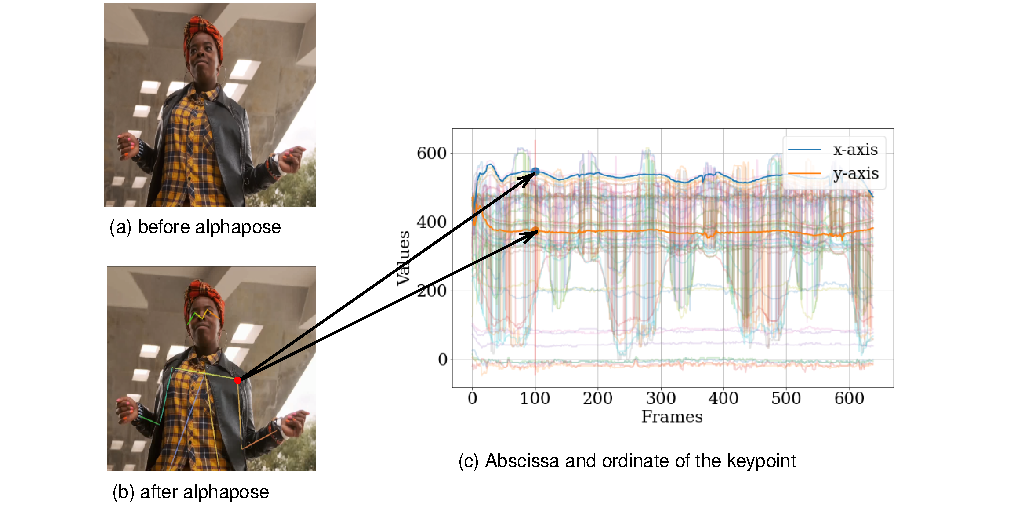
\includegraphics[width=\textwidth]{alphapose_pipeline.pdf}
	\caption{The pipeline of video processing.}
	\label{fig:alphapose_pipeline}
\end{figure}

The experiment is carried on a set of manually collected data. 
It is a collection of key points obtained from a video of a person's movement, as well as accelerometer and gyroscope readings taken from a person's hand.
The pipeline of transforming video into multidimensional time series is shown in figure \ref{fig:alphapose_pipeline}.
In the experiment, a time series forecast is constructed using the detected related components of the time series.

\section{Problem statement}
Let the values of the multivariate time series 
\[ \bS_y(t) = [S_y^1(t), \ldots, S_y^r(t)] \T \]
be available at time points $t = 1, 2, \ldots, n$.
We assume that a set of auxiliary time series $S_x^1(t), \ldots, S_x^m(t)$ affects the values of $\bS_y(t)$.

It is necessary to predict the values of the original time series $\bS_y(t)$ at time points $n+1, \ldots, n+p$.
We assume that the values of the auxiliary time series are available in the time period for which the prediction of the time series $\bS_y(t)$ is carried out.

In order to calculate the future values of a time series, we must determine a functional dependence illustrating the relationship between the past values of $\bS_y(t)$ and the future ones, as well as taking into account the influence of auxiliary time series $S_x^1(t), \ldots, S_x^m(t)$.

\begin{definition}
	\textbf{The} \emph{prediction model} \textbf{with external factors} is a function:
	\begin{equation*}
		\bS_y(t) = \bF(\bS_y(t-1), \ldots, S_x^1(t), \ldots, S_x^m(t), \ldots) + \boldsymbol{\epsilon}_t.
	\end{equation*}
\end{definition}

The algorithm of sequential locally weighted global linear map (SMAP) \cite{sugihara1994nonlinear} is used as a prediction model with external factors.

The quality criterion of the model is its mean-square error:

\begin{equation*}
	\mathcal{Q} = \dfrac{1}{p} \sum\limits_{i=n+1}^{n+p} ||\boldsymbol{\epsilon}_i||^2.
\end{equation*}

The specificity of this problem is that the size $m$ of the time series set is quite large and that among the time series $S_x^1(t), \ldots, S_x^m(t)$ there are many highly correlated ones.
As a result, using the entire set to predict the time series $\bS_y(t)$ leads to poor forecast quality.
Therefore, the following pipeline for predicting the target variable is proposed:

\begin{enumerate}
	\item Train one of the dimensionality reduction methods if it has trainable parameters.
	\item Translate the source data into latent space.
	\item Apply prediction model with external factors to latent data.
	\item (Optional) Decode obtained predictions to the target space.
\end{enumerate}

\begin{figure}[bhtp]
	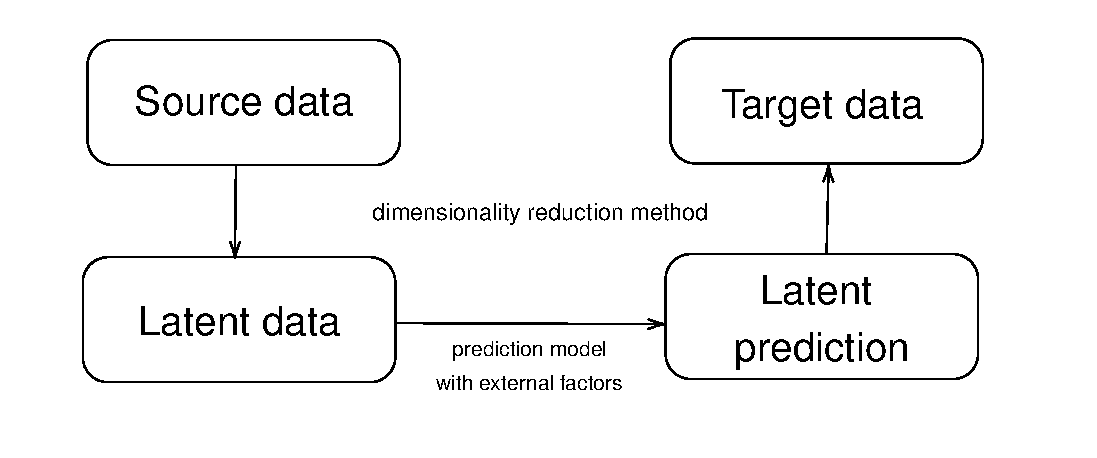
\includegraphics[width=\textwidth]{inference_pipeline}
	\caption{Inference pipeline of the prediction model}
\end{figure}


One way to project source data is to select a fixed number of time series that have the greatest impact on the target variable using the CCM method.
For a pair of time series
\begin{equation*}
	\bigl(S_x^i(t), S_y^j(t) \bigr) \quad i = 1, \ldots, m \quad j = 1, \ldots r
\end{equation*} 
it determines the impact measure of the time series $S_x^i(t)$ on the target variable $S_y^j(t)$.
Next, select the time series from the set with the maximum impact measure.

\subsection{CCM method}
\begin{figure}[bhtp]
	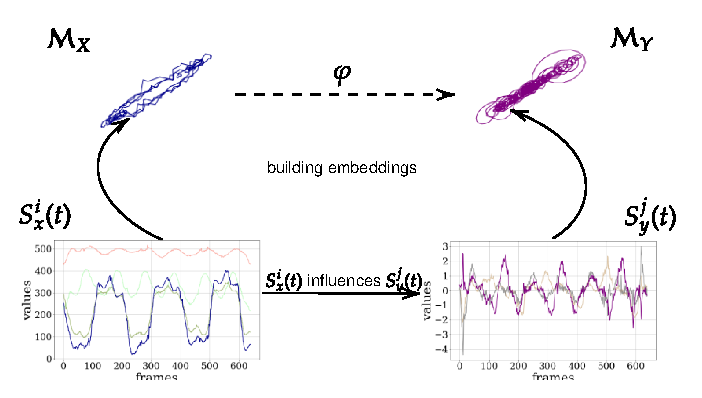
\includegraphics[width=\textwidth]{block_scheme_4.pdf}
	\caption{Application of the CCM method to select the most significant components of a time series}
	\label{fig:schema}
\end{figure}

Let's define the trajectory matrix of the time series $\bx = [x_1, \ldots, x_n]$ as follows:

\begin{equation*} \label{eq:traj_mat}
	\bH_{\bx} = \begin{bmatrix}
		x_1 & x_2 & \ldots & x_{\tau} \\
		x_2 & x_3 & \ldots & x_{\tau+1} \\
		\vdots & \vdots & \ddots & \vdots \\
		x_{N} & x_{N+1} & \ldots & x_n
	\end{bmatrix}, 
\end{equation*} 

where $N$ is the number of delays, $\tau = n - N + 1$.

Denote the $i\text{-th}$ column of the matrix $\bH_{\bx}$ by $\bx_i$.
The matrix $\bH_{\bx}$ takes the form:

\begin{equation*}\label{eq:traj_mat_short}
	\bH_{\bx} = [\bx_1, \ldots, \bx_{\tau}], \qquad \bx_i = [x_i, x_{i+1}, \ldots, x_{i+N-1}] \T
\end{equation*}

Note that all vectors $\bx_t$ belong to the $N-\text{dimensional}$ trajectory space $\dH_{\bx} \subseteq \dR^N$ of the time series $\bx$ and form the phase trajectory $\bx(t) \in \dR^N$.

To detect the relationship between the time series $\bx$ and $\by$, take the element $\bx_0$ from the trajectory space $\dH_{\bx}$ and find $k$ nearest neighbors in the same space. 
Let's denote their time indices (from near to far) by $t_1, \ldots, t_k$.

Since both time series are defined on the same timeline, then we can uniquely obtain the value of the time series $\by$ at time point $t_0 \in \{1, \ldots, n\}$ by the value of the time series $\bx$ and vice versa.
Introduce the mapping from $\dH_{\bx}$ to $\dH_{\by}$ as follows:
$$ \varphi: \bx_0 \mapsto \widehat{\by_0} = \sum\limits_{i=1}^k w_i \by_{t_i}, \qquad 
w_i = \dfrac{u_i}{\sum\limits_{j=1}^k u_j}, \qquad
u_i = \exp \bigl( - \| \bx_0 - \bx_{t_i} \| \bigr).$$

\begin{definition}
	The time series $\bx$ and $\by$ are called \textbf{linked} if the mapping $\varphi$ is Lipschitz:
	$$\rho_{\dH_{\by}}(\varphi(\bx_i), \varphi(\bx_j)) \leq C \rho_{\dH_{\bx}}(\bx_i, \bx_j) \qquad \bx_i, \bx_j \in \dH_{\bx}. $$
\end{definition}

We introduce a metric proximity function of vectors in the vicinity of $U_k(\bx_{t_0})$ and $U_k(\by_{t_0})$ to check for connectivity:

\begin{equation}
	L(\bx, \by) = \dfrac{R(U_k(\bx_{t_0}))}{R(U_k(\by_{t_0}))}, \qquad R(U_k(\bx_{t_0})) = \dfrac{1}{k} \sum\limits_{i=1}^k \rho_{\dH_{\bx}}(\bx_{t_0}, \bx_{t_j}).
\end{equation}

If $L(\bx,\by)$ is greater than the specified threshold, then the time series $\by$ depends on the time series $\bx$.

Another way to project the source data is to use the Pearson correlation coefficient $\text{corr}(\by_0, \widehat{\by_0})$. 
One can choose a fixed amount of mostly correlated auxiliary time series or filter them out using threshold.

\subsection{PLS method}
Another way to solve above stated problem is to reduce the dimension in a consistent manner.
The partial least squares method restores the relationship between the datasets $\bX$ and $\bY$.
The object matrix $\bX$ and the target matrix $\bY$ are projected onto the latent space $\dR^K$ of smaller dimension as follows:
$$ \underset{n \times d}{\bX} = \underset{n \times K}{\bT} \cdot \underset{K \times d}{\bP\T} + \underset{n \times d}{\bE} $$
$$ \underset{n \times s}{\bY} = \underset{n \times K}{\bU} \cdot \underset{K \times s}{\bQ\T} + \underset{n \times s}{\bF}, $$
where $\bT$ and $\bU$ ~--- matrices describing objects and targets in the latent space, $\bP$ and $\bQ$ --- transition matrices from the latent space to the original, $\bE$ and $\bF$ --- remainder matrices.

The source data transformation function has the form:
$$f(\bX) = \bX\bW_{\bx}\qquad g(\bY) = \bY\bW_{\by}, $$
where the weight matrices $\bW_{\bx} \in \dR^{d \times K}$ and $\bW_{\by}\in \dR^{s \times K}$ are found by maximizing the sample covariance:
$$ (\bW_{\bx}, \bW_{\by}) = \underset{\bW_{\bx}, \bW_{\by}}{\text{argmax}}\; \text{Cov}(\bX\bW_{\bx}, \bY\bW_{\by})$$

The PLS algorithm works for previously column-normalized matrices $\bX$ and $\bY$ and the number of components $K$ as follows.
Let's set $\bX_1 = \bX, \: \bY_1 = \bY$.
Next, for each $k \in [1, K]$:
\begin{enumerate}
	\item Calculate $\ba_k\in \dR^d$ and $\bb_k\in \dR^s$, the first left and right singular vectors of the matrix $\bX_k^T\bY_k$; from the definition it follows that $(\ba_k, \bb_k) = \underset{\ba, \bb}{\text{argmax}} \text{Cov} (\bX_k \ba, \bY_k \bb)$.
	\item Project the matrices $\bX_k$ and $\bY_k$ onto singular vectors: $\bt_k = \bX_k \ba_k, \; \bu_k = \bY_k\bb_k$.
	Best rank-one approximation
	\item Regress the matrix $\bX_k$ by the vector $\bt_k$, that is, find the vector $\bp_k$ such that the matrix $\bt_k\bp_k\T$ is the best rank-one approximation of the matrix $\bX_k$ by the Frobenius norm; do the same with the matrix $\bY_k$ and the vector $\bu_k$ and get the vector $\bq_k$.
	\item Subtract from the matrix $\bX_k$ its rank-one approximation from the previous step, denote this matrix $\bX_{k+1}$; similarly, get the matrix $\bY_{k+1}$.
\end{enumerate}

Get an explicit form of the matrices $\bW_{\bx}$ and $\bW_{\by}$ from the PLS algorithm. Note that:
$$\bX\cdot\bA(\bP\T\bA)^{-1} = (\bT\bP\T\bA + \bE\bA)(\bP \T \bA)^{-1} \approx\bT, $$
where the matrices $\bA, \:\bP, \:\bT$ are formed from the columns $\ba_k, \:\bp_k, \:\bt_k$ respectively. 
Similarly, $\bY\cdot\bB(\bQ\T\bB)^{-1} \approx \bU$, where the matrices $\bB, \:\bQ, \:\bU$ are formed from the columns $\bb_k, \:\bq_k, \: \bu_k$, respectively.
Thus:
$$\bW_{\bx} = \bA(\bP\T\bA)^{-1}, \qquad\bW_{\by}= \bB(\bQ\T\bB)^{-1}. $$

\subsection{PLS-Autoencoder and PLS-CCM methods}
The main disadvantage of the classical PLS method is the low quality when working with data that have complex nonlinear dependencies.
For this reason, extensions of the linear PLS method, that transform input data using smooth nonlinear functions, have been developed .

One of such extensions is the PLS-Autoencoder method.
Neural networks act as parametric functions that translate the source data into the latent space and vice versa.
Multilayer perceptrons are used in this work.

\begin{figure}
	\begin{tikzpicture}[scale=1, every node/.style={scale=1}]
		\matrix (m) [matrix of math nodes,row sep=4em,column sep=5em,minimum width=3em]
		{
			\underset{n \times d}{\bX} & \underset{n \times s}{\bY} \\
			\underset{n \times K}{\mathbf{T}} & \underset{n \times K}{\mathbf{U}} \\
		};
		\path[-stealth]
		(m-2-1) edge node [right] {$\varphi_{\text{dec}}$} (m-1-1)
		(m-2-2) edge node [left] {$\psi_{\text{dec}}$} (m-1-2)
		(m-1-1) edge [bend right] node [left] {$\varphi_{\text{enc}}$} (m-2-1)
		(m-1-2) edge [bend left] node [right] {$\psi_{\text{enc}}$} (m-2-2)
		(m-2-1) edge [<->] (m-2-2);
	\end{tikzpicture}
	\qquad
	\begin{tikzpicture}[scale=1, every node/.style={scale=1}]
		\matrix (m) [matrix of math nodes,row sep=4em,column sep=5em,minimum width=3em]
		{
			\underset{n \times d}{\bX} & \underset{n \times s}{\bY} \\
			\underset{n \times K}{\mathbf{T}} & \underset{n \times K}{\mathbf{U}} \\
		};
		\path[-stealth]
		(m-2-1) edge node [right] {$\varphi_{\text{dec}}$} (m-1-1)
		(m-2-2) edge node [left] {$\psi_{\text{dec}}$} (m-1-2)
		(m-1-1) edge [bend right] node [left] {$\varphi_{\text{enc}}$} (m-2-1)
		(m-1-2) edge [bend left] node [right] {$\psi_{\text{enc}}$} (m-2-2)
		(m-2-1) edge [->] node [above] {$CCM_{\mathbf{TU}}$} (m-2-2)
		(m-1-1) edge [->] node [above] {$CCM_{\mathbf{XY}}$} (m-1-2);
	\end{tikzpicture}
	\caption{Left: PLS-Autoencoder, right: PLS-CCM}
\end{figure}

The loss function of this model has the form:
\begin{gather*}
	\mathcal{L} = \lambda_1 \cdot \mathcal{L}^X_{\text{recov}}(\bX, \hat{\bX}) + \lambda_2 \cdot \mathcal{L}^Y_{\text{recov}}(\bY, \hat{\bY}) + \lambda_3 \cdot \mathcal{L}_{\text{cons}}(\bT, \bU), 
	\qquad \lambda_1, \lambda_2, \lambda_3 > 0,	\\
	\mathcal{L}^X_{\text{recov}}(\bX, \hat{\bX}) = \| \bX - \hat{\bX}\|_2^2 \: , \text{ where } \hat{\bX} = \varphi_{\text{dec}}(\varphi_{\text{enc}}(\bX)), \\
	\mathcal{L}^Y_{\text{recov}}(\bY, \hat{\bY}) = \| \bY - \hat{\bY}\|_2^2 \: , \text{ where } \hat{\bY} = \psi_{\text{dec}}(\psi_{\text{enc}}(\bY)), \\
	\mathcal{L}_{\text{cons}}(\bT, \bU) = \dfrac{1}{1 + \left( \frac{1}{n} \, \text{tr}\bigl(\bU_{\text{centered}}\T \bT_{\text{centered}} \bigr) \right)^2}
\end{gather*}
where $\mathcal{L}_{\text{recov}}$ is responsible for how accurately the original data is restored from their projections into the latent space, and $\mathcal{L}_{\text{cons}}$ is responsible for the connectivity of low-dimensional latent representations.

It is worth emphasizing that $\mathcal{L}_{\text{cons}}$ maximizes the sum square of the corresponding features covariance, which are columns of the matrices $\bT$ and $\bU$.
Thus, this method does not take into account the consistency of objects in the latent space, that is, rows of matrices $\bT$ and $\bU$.

The new PLS-CCM method takes into account object consistency using metric functions from the CCM method. It is an extension of PLS-Autoencoder, only a new loss function is added:
$$ \mathcal{L}_\text{oc}(\bX, \bY, \bU, \bT) = \left( CCM_{\mathbf{XY}} - CCM_{\mathbf{TU}} \right)^2 ,$$
where $CCM_{\mathbf{XY}}$ ~--- the value characterizing the quality of approximation $\by_n$ using $\bx_n$ constructed in the trajectory space consisting of the first $n-1$ objects, and $CCM_{\mathbf{TU}}$~--- the same value, obtained from the matrices $\bU$ and $\bT$.

\section{Computational experiment}
The aim of the experiment is to compare different methods of consistent dimensionality reduction of spaces.
These methods are used to predict the trajectory of the hand movement according to the corresponding video sequence.
An important experiment part is the study of the results of the time series prediction model applied to the elements of phase trajectories space and to the elements of the trajectory subspace of a smaller dimension.

\begin{figure}[bhtp]
	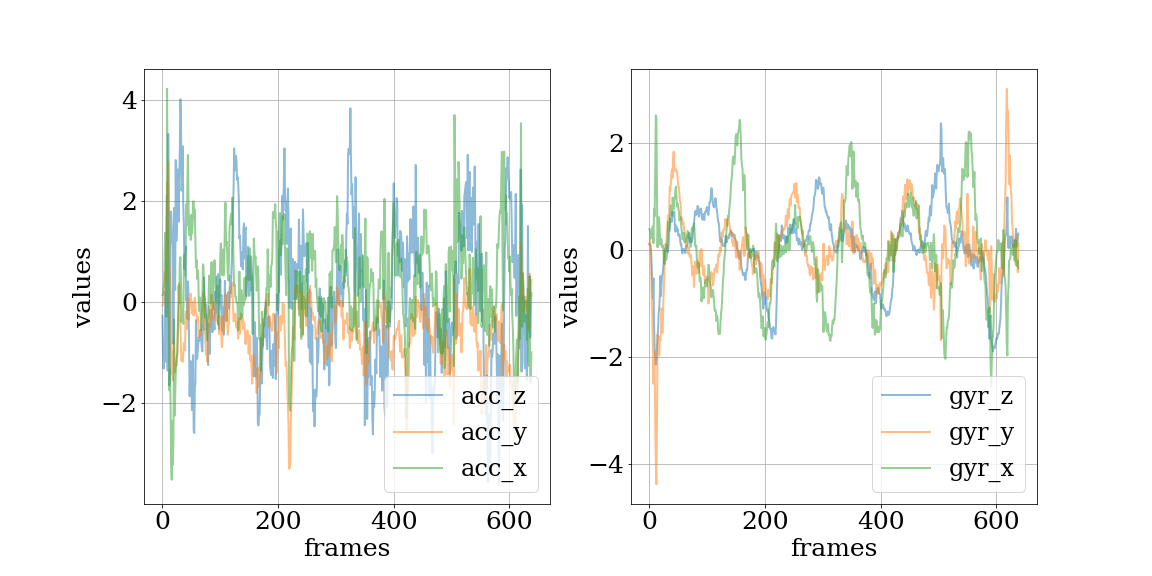
\includegraphics[width=\textwidth]{cyclic_devices_data.png}
	\caption{Accelerometer and gyroscope data obtained by hand movement}
	\label{fig:devices_data}
\end{figure}
The data is a set of videos on which various hand movements (cyclic and chaotic) are performed. 
The data also includes accelerometer and gyroscope readings with a frequency of 100 Hertz, fixed on one of the hands.
These devices form a 6-dimensional time series: The accelerometer and gyroscope show changes in values along the X, Y, and Z axes.
Next, using the alphapose framework \cite{alphapose_fang2017rmpe, alphapose_li2019crowdpose, alphapose_xiu2018poseflow}, the coordinates of the limbs, namely 68 key points, are extracted from the video sequence.
As a result, we obtain a multivariate time series of dimension 136, each component of which shows a change in one of the coordinates of some key point.
Then highly correlated components are excluded from the resulting time series.
After that, the resulting multivariate time series are reduced to one time scale by removing elements of a longer time series.

\begin{figure}[bhtp]
	\centering
	\subfloat[The result of the alphapose framework]{%
		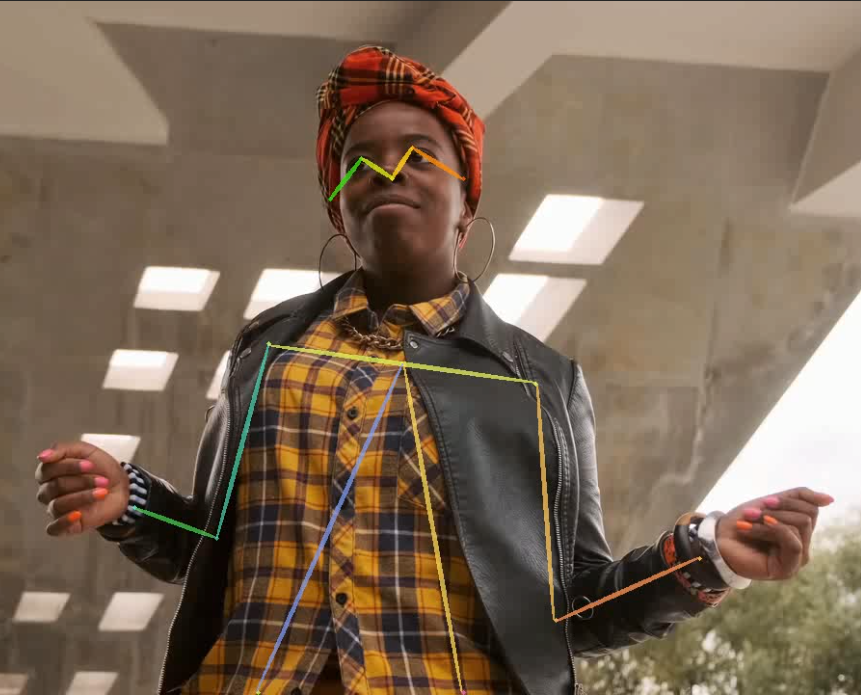
\includegraphics[width=0.45\linewidth]{after_alphapose.png}%
	}
	\subfloat[Keypoints data obtained from the video]{%
		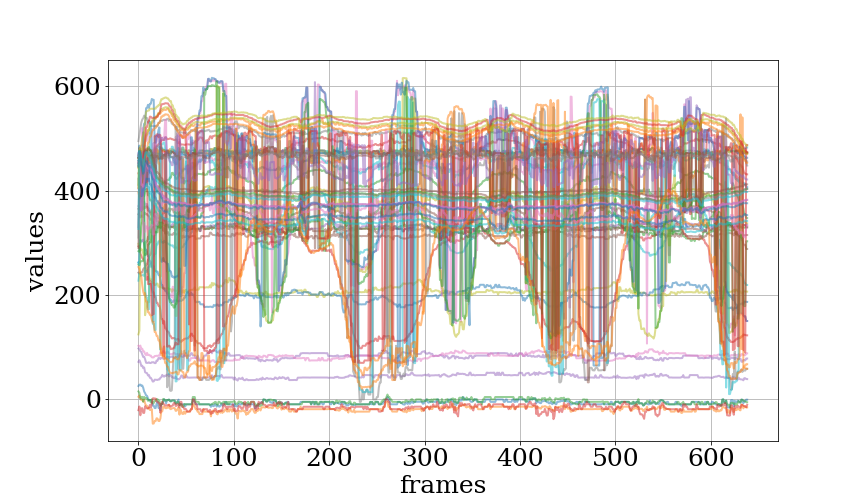
\includegraphics[width=0.45\linewidth]{cyclic_video_data.png}
	}
	\caption{Video processing scheme}
	\label{fig:video_data}
\end{figure}

\section{Error analysis}
\begin{table}[bhtp]
	\fontsize{10pt}{14pt}
	\selectfont
	\centering
	\caption{Comparison of the error (MSE) of the predictive model applied in the trajectory space and in its subspace obtained by CCM}
	\label{tbl:space_and_subspace}
	\begin{tabularx}{\textwidth}{c|XXXXXX}
		\hline
		& acc\_z & acc\_y & acc\_x & gyr\_z & gyr\_y & gyr\_x \\
		\hline
		space & 1.053 $\pm$ 2.223 & 0.401 $\pm$ 0.833 & 0.483 $\pm$ 0.825 & 0.084 $\pm$ 0.537 & 0.090 $\pm$ 0.094 & 0.063 $\pm$ 0.295 \\
		\hline
		subspace & 0.315 $\pm$ 0.461 & 0.043 $\pm$ 0.051 & 0.150 $\pm$ 0.177 & 0.001 $\pm$ 0.001	& 0.015 $\pm$ 0.031 & 0.001 $\pm$ 0.003 \\
		\hline
	\end{tabularx}
\end{table}

To begin with, let's compare the predictions quality of the forecasting model applied in the trajectory space and its subspace.
The table \ref{tbl:space_and_subspace} shows the mean-square error of the predictions of the accelerometer and gyroscope values for each of the axes and their standard deviations.
It shows that the predictive model applied in the trajectory subspace gives more accurate predictions, since most of the features of the original space are uninformative and many of them are highly correlated.

Next, we will consider various methods of dimension reduction of the trajectory space.
5 methods were compared: CCM (K video features are selected that have the greatest impact on one of the accelerometer or gyroscope readings), PLS, CCA, PLS-AE, PLS-CCM.
These methods are applied on two data sets: corresponding to cyclic and arbitrary hand movements.
In the PLS-AE and PLS-CCM methods, a multilayer perceptron with the LeakyReLU activation function is taken as encoding and recovery functions, 

\begin{table}[bhtp]
	\centering
	\caption{The standard deviation between the true readings of the devices and the predictions obtained with one of the dimensionality reduction methods}
	\label{tbl:methods}
	\begin{tabular}{l|c|lllll}
		\hline
		\multicolumn{2}{l}{\diaghead{\hskip4cm}{Target feature}{Method}} \vline & CCM & PLS & CCA & PLS-AE & PLS-CCM \\
		\hline
		\multirow{6}{*}{\rotatebox[origin=c]{90}{cyclic}} & acc\_z & 0.400 & 0.067 & 0.146 & \textbf{0.065} & 0.097 \\
		& acc\_y & \textbf{0.011} & 0.045 & 0.219 & 0.067 & 0.066 \\
		& acc\_x & {0.056} & 0.073 & 0.092 & \textbf{0.045} & 0.054 \\
		& gyr\_z & \textbf{0.001} & 0.034 & 0.105 & 0.031 & 0.018 \\
		& gyr\_y & \textbf{0.002} & 0.023 & 0.010 & 0.024 & 0.070 \\
		& gyr\_x & {0.027} & 0.045 & 0.196 & 0.011 & \textbf{0.009} \\
		\hline
		\multirow{6}{*}{\rotatebox[origin=c]{90}{chaotic}} & acc\_z & 1.015 & \textbf{0.256} & 0.405 & 0.357 & 0.325 \\
		& acc\_y & 0.547 & 0.075 & \textbf{0.036} & 0.155 & 0.156 \\
		& acc\_x & {0.568} & 0.382 & 0.628 & 0.364 & \textbf{0.324} \\
		& gyr\_z & {0.099} & 0.066 & \textbf{0.021} & 0.259 & 0.127 \\
		& gyr\_y & {0.263} & 0.032 & \textbf{0.028} & 0.103 & 0.172 \\
		& gyr\_x & {0.074} & \textbf{0.039} & 0.055 & 0.129 & 0.298 \\
		\hline   
	\end{tabular}
\end{table}

\section{Conclusion}
The paper proposes a method for generalizing the PLS and CCA methods using the Sugihara method by constructing embeddings and choosing a metric for evaluating the quality of approximation.
A computational experiment was carried out on the data of devices and video series.
It was found that the using data from the video improves the forecasting quality.
It is shown that the predictive model is less stable when it is applied in the trajectory space.

In the future, it is planned to apply the method not to two-dimensional data that correspond to regular measurements of a certain value, but to sporadic time series.
This means that the input data will be multi-index matrices.

%%===========================================================================================%%
%% If you are submitting to one of the Nature Portfolio journals, using the eJP submission   %%
%% system, please include the references within the manuscript file itself. You may do this  %%
%% by copying the reference list from your .bbl file, paste it into the main manuscript .tex %%
%% file, and delete the associated \verb+\bibliography+ commands.                            %%
%%=====================================	======================================================%%

\bibliographystyle{bst/sn-mathphys}
\bibliography{sn-bibliography}% common bib file
%% if required, the content of .bbl file can be included here once bbl is generated
%%%%%%%%%%%%%%%%%%%%%%%%%%%%%%%%%%%%%%%%%%%%%%%%%%%%%%%%%%%%%%%%%%%%%%
%%                                                                 %%
%% Please do not use \input{...} to include other tex files.       %%
%% Submit your LaTeX manuscript as one .tex document.              %%
%%                                                                 %%
%% All additional figures and files should be attached             %%
%% separately and not embedded in the \TeX\ document itself.       %%
%%                                                                 %%
%%%%%%%%%%%%%%%%%%%%%%%%%%%%%%%%%%%%%%%%%%%%%%%%%%%%%%%%%%%%%%%%%%%%%

%%\documentclass[referee,sn-basic]{sn-jnl}% referee option is meant for double line spacing

%%=======================================================%%
%% to print line numbers in the margin use lineno option %%
%%=======================================================%%

%%\documentclass[lineno,sn-basic]{sn-jnl}% Basic Springer Nature Reference Style/Chemistry Reference Style

%%======================================================%%
%% to compile with pdflatex/xelatex use pdflatex option %%
%%======================================================%%

%%\documentclass[pdflatex,sn-basic]{sn-jnl}% Basic Springer Nature Reference Style/Chemistry Reference Style

%%\documentclass[sn-basic]{sn-jnl}% Basic Springer Nature Reference Style/Chemistry Reference Style
\documentclass[bst/sn-mathphys]{sn-jnl}% Math and Physical Sciences Reference Style
%%\documentclass[sn-aps]{sn-jnl}% American Physical Society (APS) Reference Style
%%\documentclass[sn-vancouver]{sn-jnl}% Vancouver Reference Style
%%\documentclass[sn-apa]{sn-jnl}% APA Reference Style
%%\documentclass[sn-chicago]{sn-jnl}% Chicago-based Humanities Reference Style
%%\documentclass[sn-standardnature]{sn-jnl}% Standard Nature Portfolio Reference Style
%%\documentclass[default]{sn-jnl}% Default
%%\documentclass[default,iicol]{sn-jnl}% Default with double column layout

%%%% Standard Packages
\usetikzlibrary{matrix}
\usepackage{makecell}
\usepackage{subfig}
\usepackage{tabularx}
\usepackage{tabulary}

\newcommand{\bz}{\mathbf{z}}
\newcommand{\bx}{\ensuremath{\mathbf{x}}}
\newcommand{\by}{\mathbf{y}}
\newcommand{\bv}{\mathbf{v}}
\newcommand{\bw}{\mathbf{w}}
\newcommand{\ba}{\mathbf{a}}
\newcommand{\bb}{\mathbf{b}}
\newcommand{\bp}{\mathbf{p}}
\newcommand{\bq}{\mathbf{q}}
\newcommand{\bt}{\mathbf{t}}
\newcommand{\bu}{\mathbf{u}}
\newcommand{\bT}{\mathbf{T}}
\newcommand{\bX}{\mathbf{X}}
\newcommand{\bZ}{\mathbf{Z}}
\newcommand{\bS}{\mathbf{S}}
\newcommand{\bH}{\mathbf{H}}
\newcommand{\bW}{\mathbf{W}}
\newcommand{\bY}{\mathbf{Y}}
\newcommand{\bU}{\mathbf{U}}
\newcommand{\bQ}{\mathbf{Q}}
\newcommand{\bP}{\mathbf{P}}
\newcommand{\bA}{\mathbf{A}}
\newcommand{\bB}{\mathbf{B}}
\newcommand{\bC}{\mathbf{C}}
\newcommand{\bE}{\mathbf{E}}
\newcommand{\bF}{\mathbf{F}}
\newcommand{\bomega}{\boldsymbol{\omega}}
\newcommand{\btheta}{\boldsymbol{\theta}}
\newcommand{\bgamma}{\boldsymbol{\gamma}}
\newcommand{\bdelta}{\boldsymbol{\delta}}
\newcommand{\bPsi}{\boldsymbol{\Psi}}
\newcommand{\bpsi}{\boldsymbol{\psi}}
\newcommand{\bxi}{\boldsymbol{\xi}}
\newcommand{\bchi}{\boldsymbol{\chi}}
\newcommand{\bzeta}{\boldsymbol{\zeta}}
\newcommand{\blambda}{\boldsymbol{\lambda}}
\newcommand{\beps}{\boldsymbol{\varepsilon}}
\newcommand{\bZeta}{\boldsymbol{Z}}
% mathcal
\newcommand{\cX}{\mathcal{X}}
\newcommand{\cY}{\mathcal{Y}}
\newcommand{\cW}{\mathcal{W}}

\newcommand{\dH}{\mathbb{H}}
\newcommand{\dR}{\mathbb{R}}

\renewcommand{\T}{^{\mathsf{T}}}
%%%%

%%%%%=============================================================================%%%%
%%%%  Remarks: This template is provided to aid authors with the preparation
%%%%  of original research articles intended for submission to journals published 
%%%%  by Springer Nature. The guidance has been prepared in partnership with 
%%%%  production teams to conform to Springer Nature technical requirements. 
%%%%  Editorial and presentation requirements differ among journal portfolios and 
%%%%  research disciplines. You may find sections in this template are irrelevant 
%%%%  to your work and are empowered to omit any such section if allowed by the 
%%%%  journal you intend to submit to. The submission guidelines and policies 
%%%%  of the journal take precedence. A detailed User Manual is available in the 
%%%%  template package for technical guidance.
%%%%%=============================================================================%%%%

\jyear{2022}%

%% as per the requirement new theorem styles can be included as shown below
\theoremstyle{thmstyleone}%
\newtheorem{theorem}{Theorem}%  meant for continuous numbers
%%\newtheorem{theorem}{Theorem}[section]% meant for sectionwise numbers
%% optional argument [theorem] produces theorem numbering sequence instead of independent numbers for Proposition
\newtheorem{proposition}[theorem]{Proposition}% 
%%\newtheorem{proposition}{Proposition}% to get separate numbers for theorem and proposition etc.

\theoremstyle{thmstyletwo}%
\newtheorem{example}{Example}%
\newtheorem{remark}{Remark}%

\theoremstyle{thmstylethree}%
\newtheorem{definition}{Definition}%

\raggedbottom
%%\unnumbered% uncomment this for unnumbered level heads

\begin{document}

\title{Reconstruction of acceleration hand trajectory with video}

%%=============================================================%%
%% Prefix	-> \pfx{Dr}
%% GivenName	-> \fnm{Joergen W.}
%% Particle	-> \spfx{van der} -> surname prefix
%% FamilyName	-> \sur{Ploeg}
%% Suffix	-> \sfx{IV}
%% NatureName	-> \tanm{Poet Laureate} -> Title after name
%% Degrees	-> \dgr{MSc, PhD}
%% \author*[1,2]{\pfx{Dr} \fnm{Joergen W.} \spfx{van der} \sur{Ploeg} \sfx{IV} \tanm{Poet Laureate} 
%%                 \dgr{MSc, PhD}}\email{iauthor@gmail.com}
%%=============================================================%%

\author*[1]{\fnm{Eduard} \sur{Vladimirov}}\email{vladimirov.ea@phystech.edu}

\author[1]{\fnm{Roman} \sur{Isachenko}}\email{roman.isachenko@phystech.edu}
\equalcont{These authors contributed equally to this work.}

\author[1]{\fnm{Vadim} \sur{Strijov}}\email{strijov@phystech.edu}
\equalcont{These authors contributed equally to this work.}

\affil[1]{\orgname{Moscow Institute of Physics and Technology}, \orgaddress{\street{Inststitutskii per.~9}, \city{Dolgoprudny}, \postcode{141700}, \state{Moscow Region}, \country{Russia}}}

%%==================================%%
%% sample for unstructured abstract %%
%%==================================%%

\abstract{This paper investigates the problem of forecasting a time series with a complex structure. 
The complex structure means the presence of non-linear dependencies and a varying period. 
We have to find causal relationships between time series forecasts. 
In order to do this, we reduce the dimension of trajectory spaces.
The paper introduces a new way for the consistent dimensional reduction of time series. 
The proposed method combines the partial least squares method and convergent cross mapping method. 
To demonstrate the results of the work we tackle the problem of hand trajectory reconstruction with video.}

\keywords{Pose estimation, Time series, Phase trajectory, Trajectory subspace, Convergent cross mapping, Partial least squares}
%%\pacs[JEL Classification]{D8, H51}

%%\pacs[MSC Classification]{35A01, 65L10, 65L12, 65L20, 65L70}

\maketitle

\section{Introduction}

In this paper, we solve the problem of forecasting a target time series based on other time series.
The challenge is to detect relationships between time series and exclude unrelated time series from the predictive model.
Solving this problem improves model's quality.

We propose a new method for filtering multivariate time series. 
It's based on the convergent cross mapping method (CCM) or the Sugihara method \cite{Sugihara90, sugihara1990nonlinear},
which outputs the measure of the feature importance.
CCM compares the nearest neighbors in the trajectory space of the time series $\by$ obtained from the time series $\bx$.

To construct a predictive model, one has to use a trajectory matrix (or Hankel matrix) that describes the phase space of a time series.
For example, in the method of singular spectral analysis (SSA) \cite {golyandina2005ssa, golyandina2001analysis, zhigljavsky2010singular, ignatov2016har}, the time series predictive model is based on the spectral decomposition of the trajectory matrix.
In CCM, Hankel matrices are used for checking the presence of a Lipschitz mapping between trajectory spaces.

However, the dimension of the trajectory space may be extremely high, 
which leads to instability of the predictive model.
To reduce the dimension of the trajectory space by mapping a projection of the phase trajectory into some subspace. 
There is no specific way for CCM to select a subspace in which the phase trajectory is approximated.
In the paper \cite{usmanova2020sphere_regr} this problem is solved using spherical regression: the desired subspace is defined by the set of empirical directions $\{ \bx_i - \bx_j \mid i < j \}$, where $\bx_i \text{~--- elements of the trajectory space}$. 
In the work \cite{alexandrov2005automatic} automatic selection of a pair of principal components is used.
The main idea is to compare the spectral densities of the principal components. 
A simple iteration over the principal components \cite{usmanova2019dependencies} is also used.

The partial least squares method (PLS) \cite{rosipal2005overview, sun2019application} is a popular algorithm for dimensionality reduction problem. It selects the most significant features and builds new ones as their linear combination.
This allows us to obtain a simple, accurate and stable predictive model.
The canonical correlation analysis (CCA) \cite{hardoon2004canonical} is another dimensionality reduction method, which is used in medicine \cite{sadoughi2016application}, gait recognition \cite{xing2016complete} and speech enhancement \cite{benesty2018canonical}. 
It is similar to PLS except that the PLS method maximizes the covariance between projections, and the CCA method — correlation.
The disadvantage of these models is the low accuracy in estimating nonlinear dependencies between data.
The nonlinear extensions of PLS \cite{qin1992nonlinear, rosipal2011nonlinear} have been proposed.
This article uses the PLS-Autoencoder model \cite{wiering2013neural}, which converts the source data using autoencoders.

\begingroup
\renewcommand{\arraystretch}{1.5}
\begin{table}[bhtp]
	\caption{Comparison of the dimensionality reduction methods}
	\label{tbl:dim_reduction_review}
	\begin{tabulary}{\textwidth}{L|L|L|L}
		\hline
		Method name & Advantages & Disadvantages & Loss function \\
		\hline
		Projection to Latent Space methods (PLS, CCA) & Resistance to
		highly correlated features and noise in the data & Poor prediction quality when working with data with non-linear dependencies & No \\
		\hline
		Multiview (iteration through subspaces) & Simplicity of idea and implementation & Huge amount of time & No\\
%		\hline
%		Selection of a pair of principal components & TODO & TODO & No \\
		\hline
		Nonlinear extensions of PLS (PLS-Autoencoder, PLS-CCM) & Higher generalizing ability & More hyperparameters, less resistant to data noise & Yes \\
		\hline
	\end{tabulary}
\end{table}
\endgroup

This paper shows how to apply CCM to reduce the dimension of the trajectory space and how to combine the ideas of the PLS and CCM methods.
To achieve the latter goal, a new loss function for the consistency of latent projections has been introduced.

\begin{figure}
	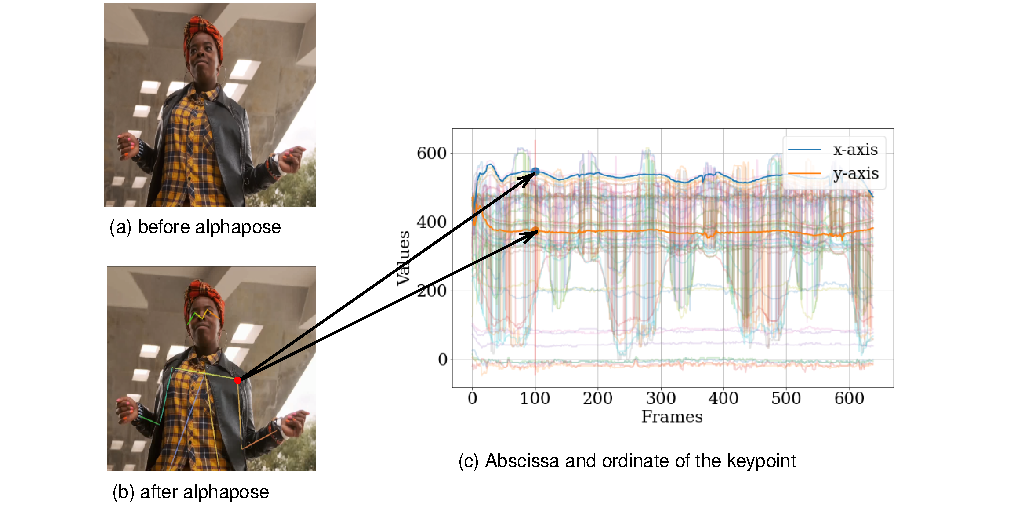
\includegraphics[width=\textwidth]{alphapose_pipeline.pdf}
	\caption{The pipeline of video processing.}
	\label{fig:alphapose_pipeline}
\end{figure}

The experiment is carried on a set of manually collected data. 
It is a collection of key points obtained from a video of a person's movement, as well as accelerometer and gyroscope readings taken from a person's hand.
The pipeline of transforming video into multidimensional time series is shown in figure \ref{fig:alphapose_pipeline}.
In the experiment, a time series forecast is constructed using the detected related components of the time series.

\section{Problem statement}
Let the values of the multivariate time series 
\[ \bS_y(t) = [S_y^1(t), \ldots, S_y^r(t)] \T \]
be available at time points $t = 1, 2, \ldots, n$.
We assume that a set of auxiliary time series $S_x^1(t), \ldots, S_x^m(t)$ affects the values of $\bS_y(t)$.

It is necessary to predict the values of the original time series $\bS_y(t)$ at time points $n+1, \ldots, n+p$.
We assume that the values of the auxiliary time series are available in the time period for which the prediction of the time series $\bS_y(t)$ is carried out.

In order to calculate the future values of a time series, we must determine a functional dependence illustrating the relationship between the past values of $\bS_y(t)$ and the future ones, as well as taking into account the influence of auxiliary time series $S_x^1(t), \ldots, S_x^m(t)$.

\begin{definition}
	\textbf{The} \emph{prediction model} \textbf{with external factors} is a function:
	\begin{equation*}
		\bS_y(t) = \bF(\bS_y(t-1), \ldots, S_x^1(t), \ldots, S_x^m(t), \ldots) + \boldsymbol{\epsilon}_t.
	\end{equation*}
\end{definition}

The algorithm of sequential locally weighted global linear map (SMAP) \cite{sugihara1994nonlinear} is used as a prediction model with external factors.

The quality criterion of the model is its mean-square error:

\begin{equation*}
	\mathcal{Q} = \dfrac{1}{p} \sum\limits_{i=n+1}^{n+p} ||\boldsymbol{\epsilon}_i||^2.
\end{equation*}

The specificity of this problem is that the size $m$ of the time series set is quite large and that among the time series $S_x^1(t), \ldots, S_x^m(t)$ there are many highly correlated ones.
As a result, using the entire set to predict the time series $\bS_y(t)$ leads to poor forecast quality.
Therefore, the following pipeline for predicting the target variable is proposed:

\begin{enumerate}
	\item Train one of the dimensionality reduction methods if it has trainable parameters.
	\item Translate the source data into latent space.
	\item Apply prediction model with external factors to latent data.
	\item (Optional) Decode obtained predictions to the target space.
\end{enumerate}

\begin{figure}[bhtp]
	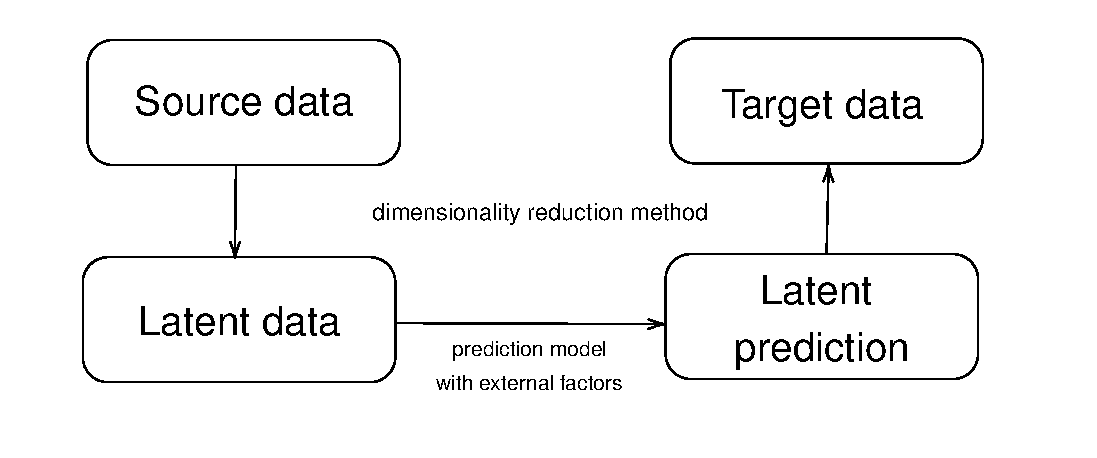
\includegraphics[width=\textwidth]{inference_pipeline}
	\caption{Inference pipeline of the prediction model}
\end{figure}


One way to project source data is to select a fixed number of time series that have the greatest impact on the target variable using the CCM method.
For a pair of time series
\begin{equation*}
	\bigl(S_x^i(t), S_y^j(t) \bigr) \quad i = 1, \ldots, m \quad j = 1, \ldots r
\end{equation*} 
it determines the impact measure of the time series $S_x^i(t)$ on the target variable $S_y^j(t)$.
Next, select the time series from the set with the maximum impact measure.

\subsection{CCM method}
\begin{figure}[bhtp]
	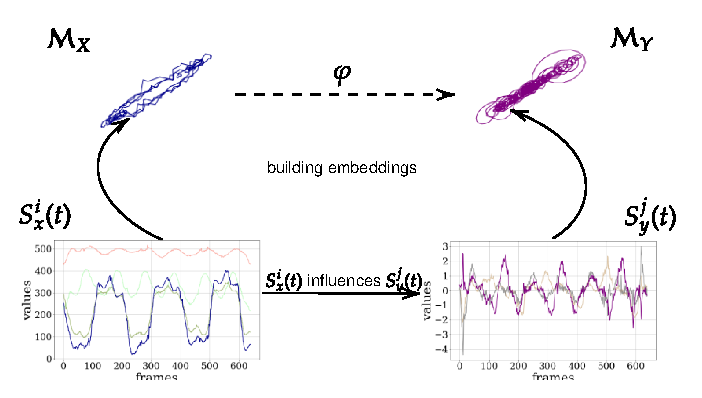
\includegraphics[width=\textwidth]{block_scheme_4.pdf}
	\caption{Application of the CCM method to select the most significant components of a time series}
	\label{fig:schema}
\end{figure}

Let's define the trajectory matrix of the time series $\bx = [x_1, \ldots, x_n]$ as follows:

\begin{equation*} \label{eq:traj_mat}
	\bH_{\bx} = \begin{bmatrix}
		x_1 & x_2 & \ldots & x_{\tau} \\
		x_2 & x_3 & \ldots & x_{\tau+1} \\
		\vdots & \vdots & \ddots & \vdots \\
		x_{N} & x_{N+1} & \ldots & x_n
	\end{bmatrix}, 
\end{equation*} 

where $N$ is the number of delays, $\tau = n - N + 1$.

Denote the $i\text{-th}$ column of the matrix $\bH_{\bx}$ by $\bx_i$.
The matrix $\bH_{\bx}$ takes the form:

\begin{equation*}\label{eq:traj_mat_short}
	\bH_{\bx} = [\bx_1, \ldots, \bx_{\tau}], \qquad \bx_i = [x_i, x_{i+1}, \ldots, x_{i+N-1}] \T
\end{equation*}

Note that all vectors $\bx_t$ belong to the $N-\text{dimensional}$ trajectory space $\dH_{\bx} \subseteq \dR^N$ of the time series $\bx$ and form the phase trajectory $\bx(t) \in \dR^N$.

To detect the relationship between the time series $\bx$ and $\by$, take the element $\bx_0$ from the trajectory space $\dH_{\bx}$ and find $k$ nearest neighbors in the same space. 
Let's denote their time indices (from near to far) by $t_1, \ldots, t_k$.

Since both time series are defined on the same timeline, then we can uniquely obtain the value of the time series $\by$ at time point $t_0 \in \{1, \ldots, n\}$ by the value of the time series $\bx$ and vice versa.
Introduce the mapping from $\dH_{\bx}$ to $\dH_{\by}$ as follows:
$$ \varphi: \bx_0 \mapsto \widehat{\by_0} = \sum\limits_{i=1}^k w_i \by_{t_i}, \qquad 
w_i = \dfrac{u_i}{\sum\limits_{j=1}^k u_j}, \qquad
u_i = \exp \bigl( - \| \bx_0 - \bx_{t_i} \| \bigr).$$

\begin{definition}
	The time series $\bx$ and $\by$ are called \textbf{linked} if the mapping $\varphi$ is Lipschitz:
	$$\rho_{\dH_{\by}}(\varphi(\bx_i), \varphi(\bx_j)) \leq C \rho_{\dH_{\bx}}(\bx_i, \bx_j) \qquad \bx_i, \bx_j \in \dH_{\bx}. $$
\end{definition}

We introduce a metric proximity function of vectors in the vicinity of $U_k(\bx_{t_0})$ and $U_k(\by_{t_0})$ to check for connectivity:

\begin{equation}
	L(\bx, \by) = \dfrac{R(U_k(\bx_{t_0}))}{R(U_k(\by_{t_0}))}, \qquad R(U_k(\bx_{t_0})) = \dfrac{1}{k} \sum\limits_{i=1}^k \rho_{\dH_{\bx}}(\bx_{t_0}, \bx_{t_j}).
\end{equation}

If $L(\bx,\by)$ is greater than the specified threshold, then the time series $\by$ depends on the time series $\bx$.

Another way to project the source data is to use the Pearson correlation coefficient $\text{corr}(\by_0, \widehat{\by_0})$. 
One can choose a fixed amount of mostly correlated auxiliary time series or filter them out using threshold.

\subsection{PLS method}
Another way to solve above stated problem is to reduce the dimension in a consistent manner.
The partial least squares method restores the relationship between the datasets $\bX$ and $\bY$.
The object matrix $\bX$ and the target matrix $\bY$ are projected onto the latent space $\dR^K$ of smaller dimension as follows:
$$ \underset{n \times d}{\bX} = \underset{n \times K}{\bT} \cdot \underset{K \times d}{\bP\T} + \underset{n \times d}{\bE} $$
$$ \underset{n \times s}{\bY} = \underset{n \times K}{\bU} \cdot \underset{K \times s}{\bQ\T} + \underset{n \times s}{\bF}, $$
where $\bT$ and $\bU$ ~--- matrices describing objects and targets in the latent space, $\bP$ and $\bQ$ --- transition matrices from the latent space to the original, $\bE$ and $\bF$ --- remainder matrices.

The source data transformation function has the form:
$$f(\bX) = \bX\bW_{\bx}\qquad g(\bY) = \bY\bW_{\by}, $$
where the weight matrices $\bW_{\bx} \in \dR^{d \times K}$ and $\bW_{\by}\in \dR^{s \times K}$ are found by maximizing the sample covariance:
$$ (\bW_{\bx}, \bW_{\by}) = \underset{\bW_{\bx}, \bW_{\by}}{\text{argmax}}\; \text{Cov}(\bX\bW_{\bx}, \bY\bW_{\by})$$

The PLS algorithm works for previously column-normalized matrices $\bX$ and $\bY$ and the number of components $K$ as follows.
Let's set $\bX_1 = \bX, \: \bY_1 = \bY$.
Next, for each $k \in [1, K]$:
\begin{enumerate}
	\item Calculate $\ba_k\in \dR^d$ and $\bb_k\in \dR^s$, the first left and right singular vectors of the matrix $\bX_k^T\bY_k$; from the definition it follows that $(\ba_k, \bb_k) = \underset{\ba, \bb}{\text{argmax}} \text{Cov} (\bX_k \ba, \bY_k \bb)$.
	\item Project the matrices $\bX_k$ and $\bY_k$ onto singular vectors: $\bt_k = \bX_k \ba_k, \; \bu_k = \bY_k\bb_k$.
	Best rank-one approximation
	\item Regress the matrix $\bX_k$ by the vector $\bt_k$, that is, find the vector $\bp_k$ such that the matrix $\bt_k\bp_k\T$ is the best rank-one approximation of the matrix $\bX_k$ by the Frobenius norm; do the same with the matrix $\bY_k$ and the vector $\bu_k$ and get the vector $\bq_k$.
	\item Subtract from the matrix $\bX_k$ its rank-one approximation from the previous step, denote this matrix $\bX_{k+1}$; similarly, get the matrix $\bY_{k+1}$.
\end{enumerate}

Get an explicit form of the matrices $\bW_{\bx}$ and $\bW_{\by}$ from the PLS algorithm. Note that:
$$\bX\cdot\bA(\bP\T\bA)^{-1} = (\bT\bP\T\bA + \bE\bA)(\bP \T \bA)^{-1} \approx\bT, $$
where the matrices $\bA, \:\bP, \:\bT$ are formed from the columns $\ba_k, \:\bp_k, \:\bt_k$ respectively. 
Similarly, $\bY\cdot\bB(\bQ\T\bB)^{-1} \approx \bU$, where the matrices $\bB, \:\bQ, \:\bU$ are formed from the columns $\bb_k, \:\bq_k, \: \bu_k$, respectively.
Thus:
$$\bW_{\bx} = \bA(\bP\T\bA)^{-1}, \qquad\bW_{\by}= \bB(\bQ\T\bB)^{-1}. $$

\subsection{PLS-Autoencoder and PLS-CCM methods}
The main disadvantage of the classical PLS method is the low quality when working with data that have complex nonlinear dependencies.
For this reason, extensions of the linear PLS method, that transform input data using smooth nonlinear functions, have been developed .

One of such extensions is the PLS-Autoencoder method.
Neural networks act as parametric functions that translate the source data into the latent space and vice versa.
Multilayer perceptrons are used in this work.

\begin{figure}
	\begin{tikzpicture}[scale=1, every node/.style={scale=1}]
		\matrix (m) [matrix of math nodes,row sep=4em,column sep=5em,minimum width=3em]
		{
			\underset{n \times d}{\bX} & \underset{n \times s}{\bY} \\
			\underset{n \times K}{\mathbf{T}} & \underset{n \times K}{\mathbf{U}} \\
		};
		\path[-stealth]
		(m-2-1) edge node [right] {$\varphi_{\text{dec}}$} (m-1-1)
		(m-2-2) edge node [left] {$\psi_{\text{dec}}$} (m-1-2)
		(m-1-1) edge [bend right] node [left] {$\varphi_{\text{enc}}$} (m-2-1)
		(m-1-2) edge [bend left] node [right] {$\psi_{\text{enc}}$} (m-2-2)
		(m-2-1) edge [<->] (m-2-2);
	\end{tikzpicture}
	\qquad
	\begin{tikzpicture}[scale=1, every node/.style={scale=1}]
		\matrix (m) [matrix of math nodes,row sep=4em,column sep=5em,minimum width=3em]
		{
			\underset{n \times d}{\bX} & \underset{n \times s}{\bY} \\
			\underset{n \times K}{\mathbf{T}} & \underset{n \times K}{\mathbf{U}} \\
		};
		\path[-stealth]
		(m-2-1) edge node [right] {$\varphi_{\text{dec}}$} (m-1-1)
		(m-2-2) edge node [left] {$\psi_{\text{dec}}$} (m-1-2)
		(m-1-1) edge [bend right] node [left] {$\varphi_{\text{enc}}$} (m-2-1)
		(m-1-2) edge [bend left] node [right] {$\psi_{\text{enc}}$} (m-2-2)
		(m-2-1) edge [->] node [above] {$CCM_{\mathbf{TU}}$} (m-2-2)
		(m-1-1) edge [->] node [above] {$CCM_{\mathbf{XY}}$} (m-1-2);
	\end{tikzpicture}
	\caption{Left: PLS-Autoencoder, right: PLS-CCM}
\end{figure}

The loss function of this model has the form:
\begin{gather*}
	\mathcal{L} = \lambda_1 \cdot \mathcal{L}^X_{\text{recov}}(\bX, \hat{\bX}) + \lambda_2 \cdot \mathcal{L}^Y_{\text{recov}}(\bY, \hat{\bY}) + \lambda_3 \cdot \mathcal{L}_{\text{cons}}(\bT, \bU), 
	\qquad \lambda_1, \lambda_2, \lambda_3 > 0,	\\
	\mathcal{L}^X_{\text{recov}}(\bX, \hat{\bX}) = \| \bX - \hat{\bX}\|_2^2 \: , \text{ where } \hat{\bX} = \varphi_{\text{dec}}(\varphi_{\text{enc}}(\bX)), \\
	\mathcal{L}^Y_{\text{recov}}(\bY, \hat{\bY}) = \| \bY - \hat{\bY}\|_2^2 \: , \text{ where } \hat{\bY} = \psi_{\text{dec}}(\psi_{\text{enc}}(\bY)), \\
	\mathcal{L}_{\text{cons}}(\bT, \bU) = \dfrac{1}{1 + \left( \frac{1}{n} \, \text{tr}\bigl(\bU_{\text{centered}}\T \bT_{\text{centered}} \bigr) \right)^2}
\end{gather*}
where $\mathcal{L}_{\text{recov}}$ is responsible for how accurately the original data is restored from their projections into the latent space, and $\mathcal{L}_{\text{cons}}$ is responsible for the connectivity of low-dimensional latent representations.

It is worth emphasizing that $\mathcal{L}_{\text{cons}}$ maximizes the sum square of the corresponding features covariance, which are columns of the matrices $\bT$ and $\bU$.
Thus, this method does not take into account the consistency of objects in the latent space, that is, rows of matrices $\bT$ and $\bU$.

The new PLS-CCM method takes into account object consistency using metric functions from the CCM method. It is an extension of PLS-Autoencoder, only a new loss function is added:
$$ \mathcal{L}_\text{oc}(\bX, \bY, \bU, \bT) = \left( CCM_{\mathbf{XY}} - CCM_{\mathbf{TU}} \right)^2 ,$$
where $CCM_{\mathbf{XY}}$ ~--- the value characterizing the quality of approximation $\by_n$ using $\bx_n$ constructed in the trajectory space consisting of the first $n-1$ objects, and $CCM_{\mathbf{TU}}$~--- the same value, obtained from the matrices $\bU$ and $\bT$.

\section{Computational experiment}
The aim of the experiment is to compare different methods of consistent dimensionality reduction of spaces.
These methods are used to predict the trajectory of the hand movement according to the corresponding video sequence.
An important experiment part is the study of the results of the time series prediction model applied to the elements of phase trajectories space and to the elements of the trajectory subspace of a smaller dimension.

\begin{figure}[bhtp]
	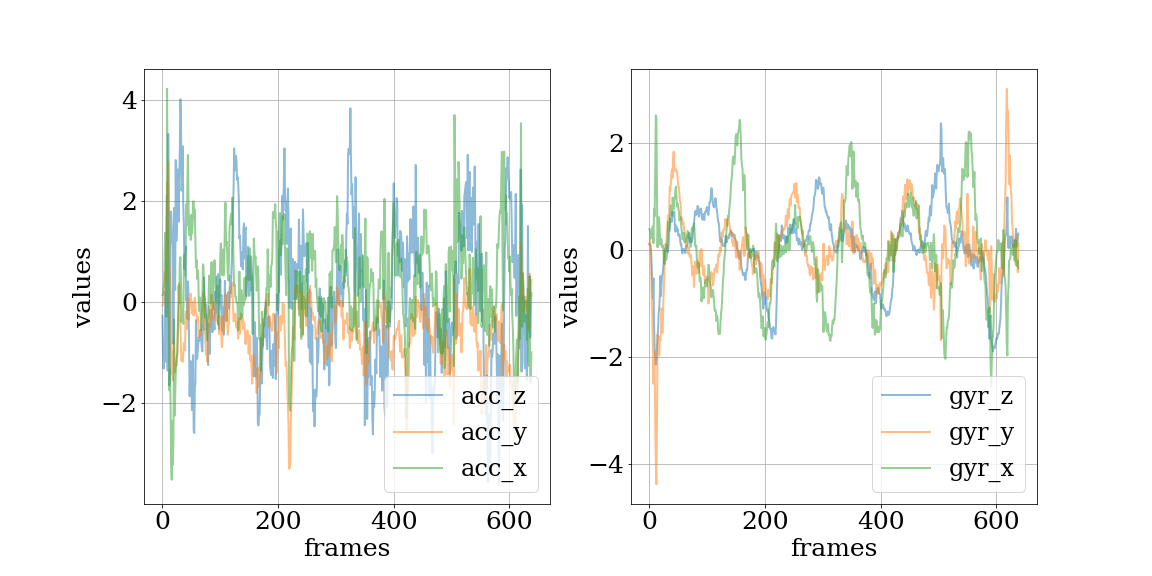
\includegraphics[width=\textwidth]{cyclic_devices_data.png}
	\caption{Accelerometer and gyroscope data obtained by hand movement}
	\label{fig:devices_data}
\end{figure}
The data is a set of videos on which various hand movements (cyclic and chaotic) are performed. 
The data also includes accelerometer and gyroscope readings with a frequency of 100 Hertz, fixed on one of the hands.
These devices form a 6-dimensional time series: The accelerometer and gyroscope show changes in values along the X, Y, and Z axes.
Next, using the alphapose framework \cite{alphapose_fang2017rmpe, alphapose_li2019crowdpose, alphapose_xiu2018poseflow}, the coordinates of the limbs, namely 68 key points, are extracted from the video sequence.
As a result, we obtain a multivariate time series of dimension 136, each component of which shows a change in one of the coordinates of some key point.
Then highly correlated components are excluded from the resulting time series.
After that, the resulting multivariate time series are reduced to one time scale by removing elements of a longer time series.

\begin{figure}[bhtp]
	\centering
	\subfloat[The result of the alphapose framework]{%
		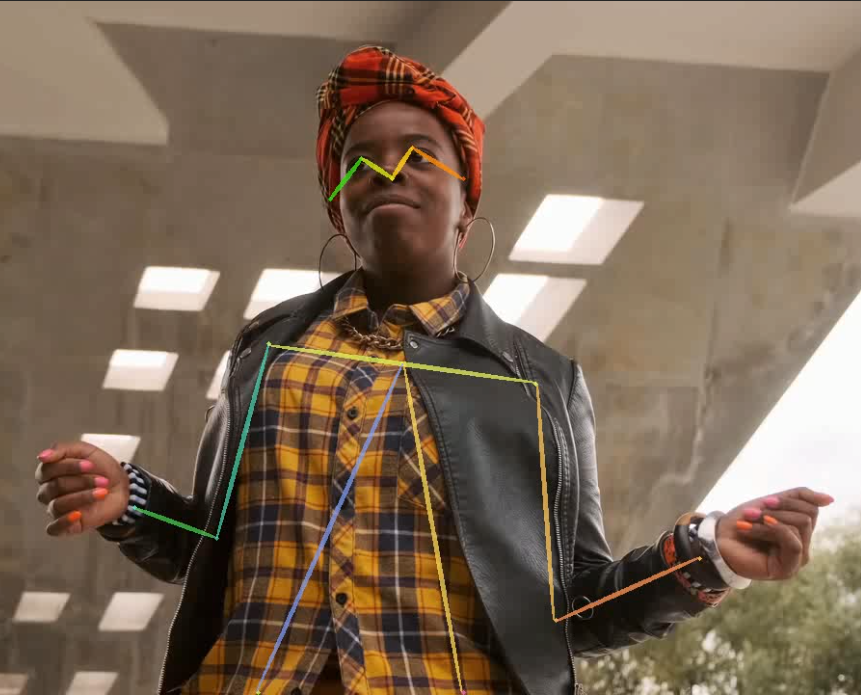
\includegraphics[width=0.45\linewidth]{after_alphapose.png}%
	}
	\subfloat[Keypoints data obtained from the video]{%
		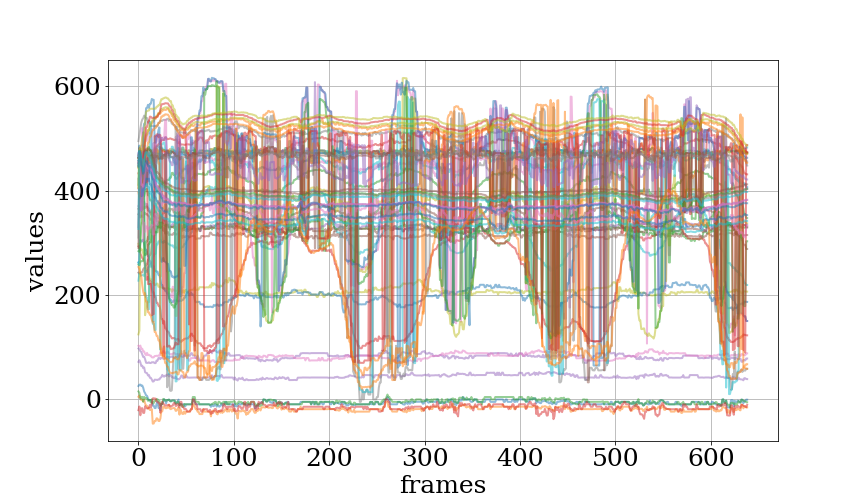
\includegraphics[width=0.45\linewidth]{cyclic_video_data.png}
	}
	\caption{Video processing scheme}
	\label{fig:video_data}
\end{figure}

\section{Error analysis}
\begin{table}[bhtp]
	\fontsize{10pt}{14pt}
	\selectfont
	\centering
	\caption{Comparison of the error (MSE) of the predictive model applied in the trajectory space and in its subspace obtained by CCM}
	\label{tbl:space_and_subspace}
	\begin{tabularx}{\textwidth}{c|XXXXXX}
		\hline
		& acc\_z & acc\_y & acc\_x & gyr\_z & gyr\_y & gyr\_x \\
		\hline
		space & 1.053 $\pm$ 2.223 & 0.401 $\pm$ 0.833 & 0.483 $\pm$ 0.825 & 0.084 $\pm$ 0.537 & 0.090 $\pm$ 0.094 & 0.063 $\pm$ 0.295 \\
		\hline
		subspace & 0.315 $\pm$ 0.461 & 0.043 $\pm$ 0.051 & 0.150 $\pm$ 0.177 & 0.001 $\pm$ 0.001	& 0.015 $\pm$ 0.031 & 0.001 $\pm$ 0.003 \\
		\hline
	\end{tabularx}
\end{table}

To begin with, let's compare the predictions quality of the forecasting model applied in the trajectory space and its subspace.
The table \ref{tbl:space_and_subspace} shows the mean-square error of the predictions of the accelerometer and gyroscope values for each of the axes and their standard deviations.
It shows that the predictive model applied in the trajectory subspace gives more accurate predictions, since most of the features of the original space are uninformative and many of them are highly correlated.

Next, we will consider various methods of dimension reduction of the trajectory space.
5 methods were compared: CCM (K video features are selected that have the greatest impact on one of the accelerometer or gyroscope readings), PLS, CCA, PLS-AE, PLS-CCM.
These methods are applied on two data sets: corresponding to cyclic and arbitrary hand movements.
In the PLS-AE and PLS-CCM methods, a multilayer perceptron with the LeakyReLU activation function is taken as encoding and recovery functions, 

\begin{table}[bhtp]
	\centering
	\caption{The standard deviation between the true readings of the devices and the predictions obtained with one of the dimensionality reduction methods}
	\label{tbl:methods}
	\begin{tabular}{l|c|lllll}
		\hline
		\multicolumn{2}{l}{\diaghead{\hskip4cm}{Target feature}{Method}} \vline & CCM & PLS & CCA & PLS-AE & PLS-CCM \\
		\hline
		\multirow{6}{*}{\rotatebox[origin=c]{90}{cyclic}} & acc\_z & 0.400 & 0.067 & 0.146 & \textbf{0.065} & 0.097 \\
		& acc\_y & \textbf{0.011} & 0.045 & 0.219 & 0.067 & 0.066 \\
		& acc\_x & {0.056} & 0.073 & 0.092 & \textbf{0.045} & 0.054 \\
		& gyr\_z & \textbf{0.001} & 0.034 & 0.105 & 0.031 & 0.018 \\
		& gyr\_y & \textbf{0.002} & 0.023 & 0.010 & 0.024 & 0.070 \\
		& gyr\_x & {0.027} & 0.045 & 0.196 & 0.011 & \textbf{0.009} \\
		\hline
		\multirow{6}{*}{\rotatebox[origin=c]{90}{chaotic}} & acc\_z & 1.015 & \textbf{0.256} & 0.405 & 0.357 & 0.325 \\
		& acc\_y & 0.547 & 0.075 & \textbf{0.036} & 0.155 & 0.156 \\
		& acc\_x & {0.568} & 0.382 & 0.628 & 0.364 & \textbf{0.324} \\
		& gyr\_z & {0.099} & 0.066 & \textbf{0.021} & 0.259 & 0.127 \\
		& gyr\_y & {0.263} & 0.032 & \textbf{0.028} & 0.103 & 0.172 \\
		& gyr\_x & {0.074} & \textbf{0.039} & 0.055 & 0.129 & 0.298 \\
		\hline   
	\end{tabular}
\end{table}

\section{Conclusion}
The paper proposes a method for generalizing the PLS and CCA methods using the Sugihara method by constructing embeddings and choosing a metric for evaluating the quality of approximation.
A computational experiment was carried out on the data of devices and video series.
It was found that the using data from the video improves the forecasting quality.
It is shown that the predictive model is less stable when it is applied in the trajectory space.

In the future, it is planned to apply the method not to two-dimensional data that correspond to regular measurements of a certain value, but to sporadic time series.
This means that the input data will be multi-index matrices.

%%===========================================================================================%%
%% If you are submitting to one of the Nature Portfolio journals, using the eJP submission   %%
%% system, please include the references within the manuscript file itself. You may do this  %%
%% by copying the reference list from your .bbl file, paste it into the main manuscript .tex %%
%% file, and delete the associated \verb+\bibliography+ commands.                            %%
%%=====================================	======================================================%%

\bibliographystyle{bst/sn-mathphys}
\bibliography{sn-bibliography}% common bib file
%% if required, the content of .bbl file can be included here once bbl is generated
%\input{Vladimirov2022RestoringHandMovementENG.bbl}

%% Default %%
%%\input sn-sample-bib.tex%

\end{document}


%% Default %%
%%\input sn-sample-bib.tex%

\end{document}


%% Default %%
%%\input sn-sample-bib.tex%

\end{document}


%% Default %%
%%\input sn-sample-bib.tex%

\end{document}
